% Options for packages loaded elsewhere
\PassOptionsToPackage{unicode}{hyperref}
\PassOptionsToPackage{hyphens}{url}
%
\documentclass[
  man,floatsintext]{apa6}
\usepackage{amsmath,amssymb}
\usepackage{lmodern}
\usepackage{iftex}
\ifPDFTeX
  \usepackage[T1]{fontenc}
  \usepackage[utf8]{inputenc}
  \usepackage{textcomp} % provide euro and other symbols
\else % if luatex or xetex
  \usepackage{unicode-math}
  \defaultfontfeatures{Scale=MatchLowercase}
  \defaultfontfeatures[\rmfamily]{Ligatures=TeX,Scale=1}
\fi
% Use upquote if available, for straight quotes in verbatim environments
\IfFileExists{upquote.sty}{\usepackage{upquote}}{}
\IfFileExists{microtype.sty}{% use microtype if available
  \usepackage[]{microtype}
  \UseMicrotypeSet[protrusion]{basicmath} % disable protrusion for tt fonts
}{}
\makeatletter
\@ifundefined{KOMAClassName}{% if non-KOMA class
  \IfFileExists{parskip.sty}{%
    \usepackage{parskip}
  }{% else
    \setlength{\parindent}{0pt}
    \setlength{\parskip}{6pt plus 2pt minus 1pt}}
}{% if KOMA class
  \KOMAoptions{parskip=half}}
\makeatother
\usepackage{xcolor}
\usepackage{graphicx}
\makeatletter
\def\maxwidth{\ifdim\Gin@nat@width>\linewidth\linewidth\else\Gin@nat@width\fi}
\def\maxheight{\ifdim\Gin@nat@height>\textheight\textheight\else\Gin@nat@height\fi}
\makeatother
% Scale images if necessary, so that they will not overflow the page
% margins by default, and it is still possible to overwrite the defaults
% using explicit options in \includegraphics[width, height, ...]{}
\setkeys{Gin}{width=\maxwidth,height=\maxheight,keepaspectratio}
% Set default figure placement to htbp
\makeatletter
\def\fps@figure{htbp}
\makeatother
\setlength{\emergencystretch}{3em} % prevent overfull lines
\providecommand{\tightlist}{%
  \setlength{\itemsep}{0pt}\setlength{\parskip}{0pt}}
\setcounter{secnumdepth}{-\maxdimen} % remove section numbering
% Make \paragraph and \subparagraph free-standing
\ifx\paragraph\undefined\else
  \let\oldparagraph\paragraph
  \renewcommand{\paragraph}[1]{\oldparagraph{#1}\mbox{}}
\fi
\ifx\subparagraph\undefined\else
  \let\oldsubparagraph\subparagraph
  \renewcommand{\subparagraph}[1]{\oldsubparagraph{#1}\mbox{}}
\fi
\newlength{\cslhangindent}
\setlength{\cslhangindent}{1.5em}
\newlength{\csllabelwidth}
\setlength{\csllabelwidth}{3em}
\newlength{\cslentryspacingunit} % times entry-spacing
\setlength{\cslentryspacingunit}{\parskip}
\newenvironment{CSLReferences}[2] % #1 hanging-ident, #2 entry spacing
 {% don't indent paragraphs
  \setlength{\parindent}{0pt}
  % turn on hanging indent if param 1 is 1
  \ifodd #1
  \let\oldpar\par
  \def\par{\hangindent=\cslhangindent\oldpar}
  \fi
  % set entry spacing
  \setlength{\parskip}{#2\cslentryspacingunit}
 }%
 {}
\usepackage{calc}
\newcommand{\CSLBlock}[1]{#1\hfill\break}
\newcommand{\CSLLeftMargin}[1]{\parbox[t]{\csllabelwidth}{#1}}
\newcommand{\CSLRightInline}[1]{\parbox[t]{\linewidth - \csllabelwidth}{#1}\break}
\newcommand{\CSLIndent}[1]{\hspace{\cslhangindent}#1}
\ifLuaTeX
\usepackage[bidi=basic]{babel}
\else
\usepackage[bidi=default]{babel}
\fi
\babelprovide[main,import]{english}
% get rid of language-specific shorthands (see #6817):
\let\LanguageShortHands\languageshorthands
\def\languageshorthands#1{}
% Manuscript styling
\usepackage{upgreek}
\captionsetup{font=singlespacing,justification=justified}

% Table formatting
\usepackage{longtable}
\usepackage{lscape}
% \usepackage[counterclockwise]{rotating}   % Landscape page setup for large tables
\usepackage{multirow}		% Table styling
\usepackage{tabularx}		% Control Column width
\usepackage[flushleft]{threeparttable}	% Allows for three part tables with a specified notes section
\usepackage{threeparttablex}            % Lets threeparttable work with longtable

% Create new environments so endfloat can handle them
% \newenvironment{ltable}
%   {\begin{landscape}\centering\begin{threeparttable}}
%   {\end{threeparttable}\end{landscape}}
\newenvironment{lltable}{\begin{landscape}\centering\begin{ThreePartTable}}{\end{ThreePartTable}\end{landscape}}

% Enables adjusting longtable caption width to table width
% Solution found at http://golatex.de/longtable-mit-caption-so-breit-wie-die-tabelle-t15767.html
\makeatletter
\newcommand\LastLTentrywidth{1em}
\newlength\longtablewidth
\setlength{\longtablewidth}{1in}
\newcommand{\getlongtablewidth}{\begingroup \ifcsname LT@\roman{LT@tables}\endcsname \global\longtablewidth=0pt \renewcommand{\LT@entry}[2]{\global\advance\longtablewidth by ##2\relax\gdef\LastLTentrywidth{##2}}\@nameuse{LT@\roman{LT@tables}} \fi \endgroup}

% \setlength{\parindent}{0.5in}
% \setlength{\parskip}{0pt plus 0pt minus 0pt}

% Overwrite redefinition of paragraph and subparagraph by the default LaTeX template
% See https://github.com/crsh/papaja/issues/292
\makeatletter
\renewcommand{\paragraph}{\@startsection{paragraph}{4}{\parindent}%
  {0\baselineskip \@plus 0.2ex \@minus 0.2ex}%
  {-1em}%
  {\normalfont\normalsize\bfseries\itshape\typesectitle}}

\renewcommand{\subparagraph}[1]{\@startsection{subparagraph}{5}{1em}%
  {0\baselineskip \@plus 0.2ex \@minus 0.2ex}%
  {-\z@\relax}%
  {\normalfont\normalsize\itshape\hspace{\parindent}{#1}\textit{\addperi}}{\relax}}
\makeatother

% \usepackage{etoolbox}
\makeatletter
\patchcmd{\HyOrg@maketitle}
  {\section{\normalfont\normalsize\abstractname}}
  {\section*{\normalfont\normalsize\abstractname}}
  {}{\typeout{Failed to patch abstract.}}
\patchcmd{\HyOrg@maketitle}
  {\section{\protect\normalfont{\@title}}}
  {\section*{\protect\normalfont{\@title}}}
  {}{\typeout{Failed to patch title.}}
\makeatother

\usepackage{xpatch}
\makeatletter
\xapptocmd\appendix
  {\xapptocmd\section
    {\addcontentsline{toc}{section}{\appendixname\ifoneappendix\else~\theappendix\fi\\: #1}}
    {}{\InnerPatchFailed}%
  }
{}{\PatchFailed}
\keywords{keywords}
\usepackage{csquotes}
\ifLuaTeX
  \usepackage{selnolig}  % disable illegal ligatures
\fi
\IfFileExists{bookmark.sty}{\usepackage{bookmark}}{\usepackage{hyperref}}
\IfFileExists{xurl.sty}{\usepackage{xurl}}{} % add URL line breaks if available
\urlstyle{same} % disable monospaced font for URLs
\hypersetup{
  pdftitle={Do expert pianists adapt their pedagogical demonstrations to novices' skills?},
  pdfauthor={Atsuko Tominaga1, Günther Knoblich1, \& Natalie Sebanz1},
  pdflang={en-EN},
  pdfkeywords={keywords},
  hidelinks,
  pdfcreator={LaTeX via pandoc}}

\title{Do expert pianists adapt their pedagogical demonstrations to novices' skills?}
\author{Atsuko Tominaga\textsuperscript{1}, Günther Knoblich\textsuperscript{1}, \& Natalie Sebanz\textsuperscript{1}}
\date{}


\shorttitle{Do expert pianists adapt their pedagogical demonstrations to novices' skills?}

\authornote{

The authors made the following contributions. Atsuko Tominaga: Conceptualization, Methodology, Software, Formal analysis, Data curation, Visualisation, Writing - Original Draft Preparation, Writing - Review \& Editing; Günther Knoblich: Conceptualization, Methodology, Resources, Writing - Review \& Editing, Supervision, Funding acquisition; Natalie Sebanz: Conceptualization, Methodology, Resources, Writing - Review \& Editing, Supervision, Funding acquisition.

Correspondence concerning this article should be addressed to Atsuko Tominaga, Quellenstraße 51, 1100 Vienna, Austria. E-mail: \href{mailto:tominaga_atsuko@phd.ceu.edu}{\nolinkurl{tominaga\_atsuko@phd.ceu.edu}}

}

\affiliation{\vspace{0.5cm}\textsuperscript{1} Department of Cognitive Science, Central European University}

\begin{document}
\maketitle

\hypertarget{introduction}{%
\section{Introduction}\label{introduction}}

Effective teaching involves experts and novices dynamically interacting with each other (Byrne \& Rapaport, 2011). First, experts demonstrate what novices are meant to acquire and then novices attempt to reproduce what the experts demonstrated. During a skill acquisition process, experts regularly monitor novices' actions and intervene by adapting their behaviour to novices' observed abilities (Mermelshtine, 2017). This interactive learning process will be iterated until novices can perform independently without the help of experts. Experts scaffold novices' learning by identifying novices' specific problems from their unsuccessful attempts and modifying their behaviour accordingly (Ugur, Nagai, Celikkanat, \& Oztop, 2015; Zukow-Goldring \& Arbib, 2007).

Exaggeration of movement is often used to signal a communicative intent to others during real-time interactions (Pezzulo et al., 2019), including teaching contexts. When mothers were teaching how to use a novel toy to their infants, they tended to demonstrate slowly and to produce wide and expansive movements compared to when they were demonstrating to adults (Brand, Baldwin, \& Ashburn, 2002). Such pedagogical action modulations are sensitive to the skill level of learners. For instance, evidence from parental scaffolding research suggests that caregivers scaffold infants' learning when the infants failed to produce an expected action (Wood \& Middleton, 1975; Zukow-Goldring \& Arbib, 2007). Fukuyama et al. (2015) performed a study, where mothers were asked to demonstrate a cup-nesting task to their infants. There were four cups of different colours and sizes. Mothers demonstrated how to stack and fit the nesting cups with the intention to teach their infants to reproduce the actions by themselves. It was found that mothers dynamically modulated their demonstrations according to the infants' object manipulation skills. Specifically, mothers exaggerated their movements when their infants failed to produce expected actions but did not produce such exaggerations when their infants lacked the motor skills to produce the required actions. Movement exaggerations for the purpose of teaching are observed not only towards infant learners but also when knowledgeable adults are interacting with adult learners (McEllin, Knoblich, \& Sebanz, 2017). For example, participants demonstrating to a learner how to play a particular melody on a xylophone increased the amplitude of their movements, compared to playing the same melody on their own. However, it has not been established whether and how experts teaching skills to adult learners adjust their demonstrations as a function of the learners' demonstrated skills.

To address this question, we investigated whether and how experts can exaggerate specific parameters of the action to be acquired depending on learners' skill level. We chose to study expressive music performance, in which experts need to modulate multiple performance parameters such as articulation and dynamics to implement expression (Cancino-Chacón, Grachten, Goebl, \& Widmer, 2018). Musicians can create their unique expression and interpretation of music even if they play exactly the same piece because when and how they change multiple performance parameters are different. By studying expressive performance, we can investigate how precisely experts can highlight specific parameters in a multidimentional space of expression (e.g., tempo, articulation dynamics) depending on the goal of teaching (e.g., to teach articulation or dynamics) even when they are performing the same piece.

In our previous research (Tominaga, Knoblich, \& Sebanz, 2022), we demonstrated that expert pianists modulated their performance when they were asked to teach musical expressive techniques such as articulation and dynamics. In particular, expert pianists exaggerated the contrast between different dynamics (i.e., they made a larger contrast between forte and piano) when they had the intention to demonstrate dynamics. When they had the intention to demonstrate articulation, they exaggerated articulation by producing shorter staccato. In that study, experts were instructed to teach techniques to hypothetical learners and they did not hear novices' particular performances. This leaves open the question of whether experts would make specific adjustments depending on learners' skills in the way mothers have been shown to adapt demonstrations of actions to their infants' skills. If experts modulate their demonstrations based on learners' skills, their exaggeration of particular aspects should depend on the learners' actual performance with regard to the techniques to be acquired. For example, if learners did not implement notated articulation during their performance, experts should exaggerate the performance relevant to articulation. However, if learners implemented notated articulation correctly, experts should not exaggerate the performance relevant to articulation.

To obtain experimental control over learners' demonstrated proficiency in implementing particular techniques, we generated artificial recordings of novice piano performances instead of recruiting actual novice pianists. The recordings were made based on the performance data from our previous study (Tominaga et al., 2022). All the recordings were of the same piece but the recordings differed in the implementation of articulation and dynamics. According to the notated expressions in the sheet music, the proper performance of the piece required specific modulations with respect to both articulation and dynamics (\emph{Fig \ref{fig:stim}}). We generated four types of recordings. In one quarter of the recordings, both techniques were implemented; in one quarter, neither articulation nor dynamics was implemented; in the two remaining quarters, the piece was played with either only articulation or only dynamics implemented. This allowed us to investigate whether expert pianists in the role of teachers would make specific adjustments in response to the learners' demonstrated skills.

We hypothesised that expert pianists would exaggerate their performance only when specific techniques (i.e., either articulation or dynamics, or both) were missing in the recordings. More precisely, expert pianists would exaggerate articulation (i.e., producing longer legato and shorter staccato) when articulation was not implemented in the recordings whereas expert pianists would exaggerate dynamics (i.e., producing louder forte and softer piano, and larger contrast between forte and piano) when dynamics was not implemented in the recordings. If both articulation and dynamics were missing, we predicted that expert pianists would exaggerate both aspects.

\hypertarget{methods}{%
\subsection{Methods}\label{methods}}

\hypertarget{participants}{%
\subsection{Participants}\label{participants}}

We recruited 20 participants who already had a degree (above bachelor's or equivalent) in piano performance/teaching or were studying advanced piano performance at a music school. Most participants were right-handed (left: 2, ambidextrous: 2). The mean age of the participants was 28.25 years (\emph{SD} = 10.95). They had 21.55 years of practice on average (\emph{SD} = 11.59). 17 participants had teaching experience in piano (\emph{M} = 7 years, \emph{SD} = 6.68). All participants were recruited through an online participant platform (SONA system, \url{https://www.sona-systems.com}). The study (No.~2020/05) was approved by CEU PU's Psychological Research Ethics Board (PREBO).

\hypertarget{apparatus-and-stimuli}{%
\subsection{Apparatus and stimuli}\label{apparatus-and-stimuli}}

The experiment was programmed in Max/MSP (8.1.11; \url{https://cycling74.com/products/max}) on a Mac Book Pro with Mac OS X Catalina 10.15.7. A weighted Yamaha MIDI digital piano was used to record participants' performances. The pitch, onset and offset time of each note, and key velocity profiles were obtained from MIDI data using Max/MSP patchers. All auditory feedback was given to participants through headphones (Audio-Technica ATH-M50X). Sheet music was displayed on a computer monitor in front of the participants.

The recorded performances serving as stimuli were all of one piece of music that had already been used in our previous study (Tominaga et al., 2022). The piece was an excerpt from Clementi's Sonatina Op.36 (No.3) in C major. The first 12 measures of the original piece were used and modified so that the piece had an almost equal number of data points (i.e., the number of notes, the number of intervals between notes) for each dependent variable. The modified piece consisted of a 12-measure isochronous melody notated in 4/4 meter to be played with the right hand only. Two expressive notations (i.e., articulation and dynamics) were added, as shown in \emph{Fig \ref{fig:stim}}.

We created artificial recordings of novices to manipulate the displayed proficiency with regard to the two relevant techniques. There were four types of recordings: 1) recordings where both articulation and dynamics were implemented (both), 2) recordings where only articulation was implemented whereas dynamics was missing (art only), 3) recordings where only dynamics was implemented whereas articulation was missing (dyn only), and 4) recordings where neither articulation nor dynamics was implemented (none). We generated 4 instances for each type, therefore there were 16 stimuli (i.e., recordings) in total. How we generated the recordings is described in \emph{Supplementary Material}.

\begin{figure}
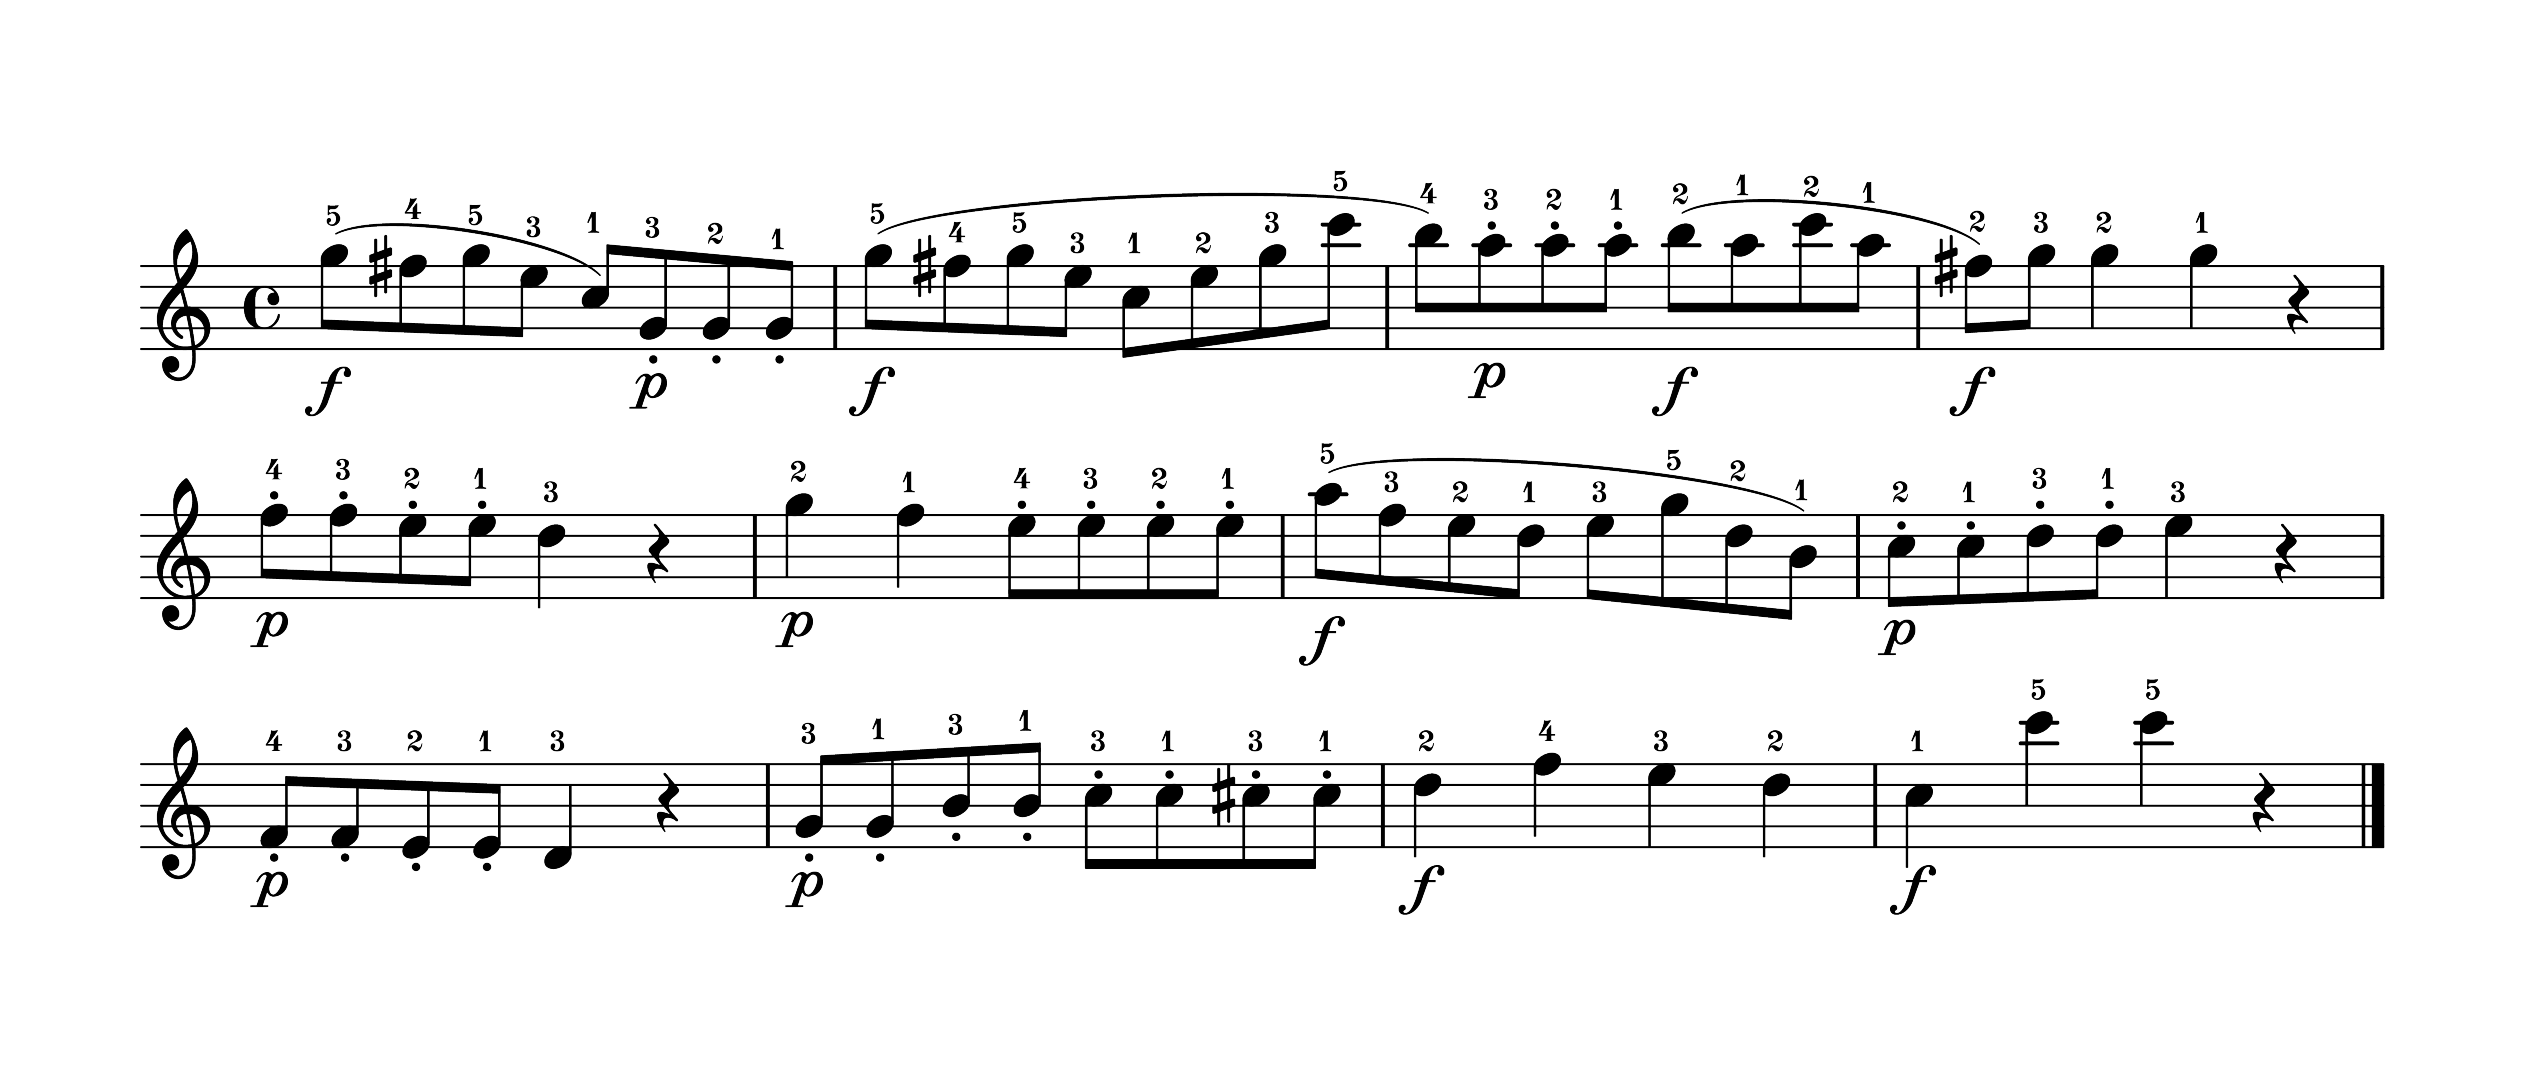
\includegraphics[width=1\linewidth]{manuscript_files/figure-latex/stimli-1} \caption{\label{fig:stim}Sheet music. For articulation notation, the curved line (slur) indicates legato and the dots indicate staccato. For dynamics notation, the symbol `f' denotes forte and the symbol `p' denotes piano. For data analysis, only the 8th notes with expressive notations were included.}\label{fig:stimli}
\end{figure}

\hypertarget{procedure}{%
\subsection{Procedure}\label{procedure}}

Prior to the experiment, participants were required to memorise the piece so that they could perform it with the notated expressions and without pitch errors in the experiment.

First, we recorded participants' baseline performance by asking them to perform the piece without having listened to any novices' performance. A leading metronome (100 quarter beats per minute, 8 beats) was given before participants started performing the piece. Sheet music (\emph{Fig \ref{fig:stim}}) was displayed in front of the participants. They were told to perform the piece expressively with their interpretation and to do their best as a performer. This instruction was given to make sure that they paid attention to the expressive aspects of the performance but did not have the intention to teach. Each participant performed the piece twice.

After we recorded the participants' baseline performance, participants were told that they were going to listen to a number of recordings from 16 different students, who were learning musical expressive techniques. Participants were required to listen to each student's recording first, and then to perform the same piece to teach musical expressive techniques to that student. In total, there were 16 trials and participants played the piece for each student only once. The order of the recordings was randomised for each participant. A leading metronome (100 quarter beats per minute, 8 beats) was given before participants started performing the piece.

After participants completed the 16 trials, they were asked to perform the piece with the same instruction as in their baseline performance. At the end of the experiment, participants filled in a questionnaire asking about their demographic information and experience in piano performance/teaching. All participants were fully debriefed at the end of the experiment and informed that the recordings had been artificially generated.

\hypertarget{data-analysis}{%
\subsection{Data analysis}\label{data-analysis}}

The dependent variables were computed from MIDI data for data analysis. Key-overlap time (KOT) is the difference between the offset time (i.e., key release time) of the current tone and the onset time of the ensuing tone and is a measure for the smoothness of musical sequences. A positive value indicates smooth legato style due to overlap between the current and ensuing tone whereas a negative value indicates sharp staccato style due to separation between the current and ensuing note. Tone intensity is assessed by key velocity (KV) and measures the loudness of a musical note. A higher value indicates forte style whereas a lower value indicates piano style. The value of KV in MIDI varies between 0 (minimum) and 127 (maximum). Also, KV difference was calculated by subtracting the KV value of the current note from that of the following note. We particularly focused on specific points where each subcomponent changed from one to the other (i.e., forte to piano or piano to forte) to measure dynamics contrast between forte and piano. Interonset intervals (IOIs) are the intervals between onsets of adjacent notes and provide a measure of tempo.

Data processing and statistical analysis were performed in R version 4.0.5. For statistical analysis, we included 8th notes with expressive notations only. Pitch errors were identified by comparing the sequence of musical notes produced by a participant with the sequence of musical notes according to the sheet music. Pitch errors included extra, missing or substituted tones and were manually removed by using the \emph{editData} R package. For note onsets, 31.87 \% of the trials contained at least one pitch error (extra notes: 5.94 \%, missing notes: 24.38 \%, substituted notes: 1.56 \%). For note offsets, 35.31 \% of the trials contained at least one pitch error (extra notes: 5.94 \%, missing notes: 24.38 \%, substituted notes: 5 \%). We found that some participants did not precisely follow the sheet music (e.g., they held some notes longer than notated), therefore the order of offsets did not correspond to that of onsets. We considered these as errors and removed the erroneous notes even if the order of onsets was correct. As a result, less than 1 \% of total responses were removed. After removing pitch errors, we removed outliers for KOT, KV, KV Difference and IOIs, defined as values more than 3 standard deviations from the mean of each dependent variable. For each dependent variable, this resulted in less than 2 \% of overall responses being removed as outliers.

First, we performed a 2 x 2 repeated-measures analysis of variance (ANOVA) with the factors Articulation (present vs.~absent) and Dynamics (present vs absent) for each dependent variable (i.e.., KOT, KV, KV Difference, IOIs). The \emph{aov\_ez} function in the \emph{afex} R package was used for a repeated-measures ANOVA. For post-hoc comparisons on the estimated marginal means, we used the \emph{emmeans} R package.

In order to investigate how their performances during the experiment differed from their baseline performances (i.e., performances that participants produced for non-teaching purposes), we performed one-way repeated-measures ANOVAs. For KOT, KV and KV Difference, we performed ANOVAs separately for each subcomponent (i.e., Legato, Staccato, Forte, Piano). The results are described in \emph{Supplementary Material}.

\hypertarget{results}{%
\section{Results}\label{results}}

All effects are reported as significant at \emph{p} \textless{} .05. For KOT, KV and KV Difference, we performed two-way ANOVAs separately for each subcomponent (i.e., legato, staccato, forte, piano).

\hypertarget{kot}{%
\subsection{KOT}\label{kot}}

\hypertarget{legato}{%
\subsubsection{Legato}\label{legato}}

As predicted, experts produced longer legato when listening to the recordings where articulation was not implemented (\emph{Fig \ref{fig:kot-1}}, left). Accordingly, there was a significant main effect of Articulation (\emph{F}(1, 19) = 5.59, \emph{p} = 0.029, \(\eta_G^2\) = 0.002). There was no significant main effect of Dynamics (\emph{F}(1, 19) = 0.06, \emph{p} = 0.81, \(\eta_G^2\) = 0.000) and no significant interaction between Articulation and Dynamics (\emph{F}(1, 19) = 1.89, \emph{p} = 0.19, \(\eta_G^2\) = 0.002).

\hypertarget{staccato}{%
\subsubsection{Staccato}\label{staccato}}

In line with our prediction, experts produced shorter staccato when listening to the recordings where articulation was not implemented (\emph{Fig \ref{fig:kot-1}}, right). Accordingly, there was a significant main effect of Articulation (\emph{F}(1, 19) = 4.88, \emph{p} = 0.040, \(\eta_G^2\) = 0.009). There was no significant main effect of Dynamics (\emph{F}(1, 19) = 0.68, \emph{p} = 0.42, \(\eta_G^2\) = 0.000) and no significant interaction between Articulation and Dynamics (\emph{F}(1, 19) = 3.13, \emph{p} = 0.093, \(\eta_G^2\) = 0.001).

\hypertarget{kv}{%
\subsection{KV}\label{kv}}

\hypertarget{forte}{%
\subsubsection{Forte}\label{forte}}

Unlike our prediction, experts did not change their performances in terms of notated forte depending on the type of recordings (\emph{Fig \ref{fig:vel-1}}, left). Neither the main effect of Articulation (\emph{F}(1, 19) = 1.66, \emph{p} = 0.21, \(\eta_G^2\) = 0.00) nor the main effect of Dynamics (\emph{F}(1, 19) = 0.33, \emph{p} = 0.57, \(\eta_G^2\) = 0.000) nor the interaction between Articulation and Dynamics was significant (\emph{F}(1, 19) = 0.00, \emph{p} = 0.96, \(\eta_G^2\) = 0.000).

\hypertarget{piano}{%
\subsubsection{Piano}\label{piano}}

Experts produced softer piano only when listening to the recordings where articulation was implemented (\emph{Fig \ref{fig:vel-1}}, right). There was a significant main effect of Articulation (\emph{F}(1, 19) = 7.18, \emph{p} = 0.01, \(\eta_G^2\) = 0.060). However, there was no significant main effect of Dynamics (\emph{F}(1, 19) = 1.80, \emph{p} = 0.20, \(\eta_G^2\) = 0.003) and no significant interaction between Articulation and Dynamics (\emph{F}(1, 19) = 0.04, \emph{p} = 0.85, \(\eta_G^2\) = 0.000).

\hypertarget{kv-difference}{%
\subsection{KV Difference}\label{kv-difference}}

Unlike our prediction, experts did not change their performances in terms of dynamics contrast depending on the type of recordings (\emph{Fig \ref{fig:vel-diff-1}}).

\hypertarget{forte-to-piano}{%
\subsubsection{Forte to Piano}\label{forte-to-piano}}

Neither the main effect of Articulation (\emph{F}(1, 19) = 3.40, \emph{p} = 0.081, \(\eta_G^2\) = 0.012) nor Dynamics (\emph{F}(1, 19) = 1.58, \emph{p} = 0.22, \(\eta_G^2\) = 0.002) nor the interaction between Articulation and Dynamics was significant (\emph{F}(1, 19) = 0.97, \emph{p} = 0.336, \(\eta_G^2\) = 0.001).

\hypertarget{piano-to-forte}{%
\subsubsection{Piano to Forte}\label{piano-to-forte}}

Neither the main effect of Articulation (\emph{F}(1, 19) = 2.25, \emph{p} = 0.150, \(\eta_G^2\) = 0.005) nor Dynamics (\emph{F}(1, 19) = 3.76, \emph{p} = 0.07, \(\eta_G^2\) = 0.004) nor the interaction between Articulation and Dynamics was significant (\emph{F}(1, 19) = 1.08, \emph{p} = 0.31, \(\eta_G^2\) = 0.001).

\hypertarget{iois}{%
\subsection{IOIs}\label{iois}}

Unlike our prediction, experts did not change the tempo depending on the type of recordings (\emph{Fig \ref{fig:ioi-1}}). Neither the main effect of Articulation (\emph{F}(1, 19) = 2.79, \emph{p} = 0.111, \(\eta_G^2\) = 0.010) nor the main effect of Dynamics (\emph{F}(1, 19) = 3.27, \emph{p} = 0.086, \(\eta_G^2\) = 0.003) nor the interaction between Articulation and Dynamics was significant (\emph{F}(1, 19) = 1.48, \emph{p} = 0.24, \(\eta_G^2\) = 0.002).

\begin{figure}
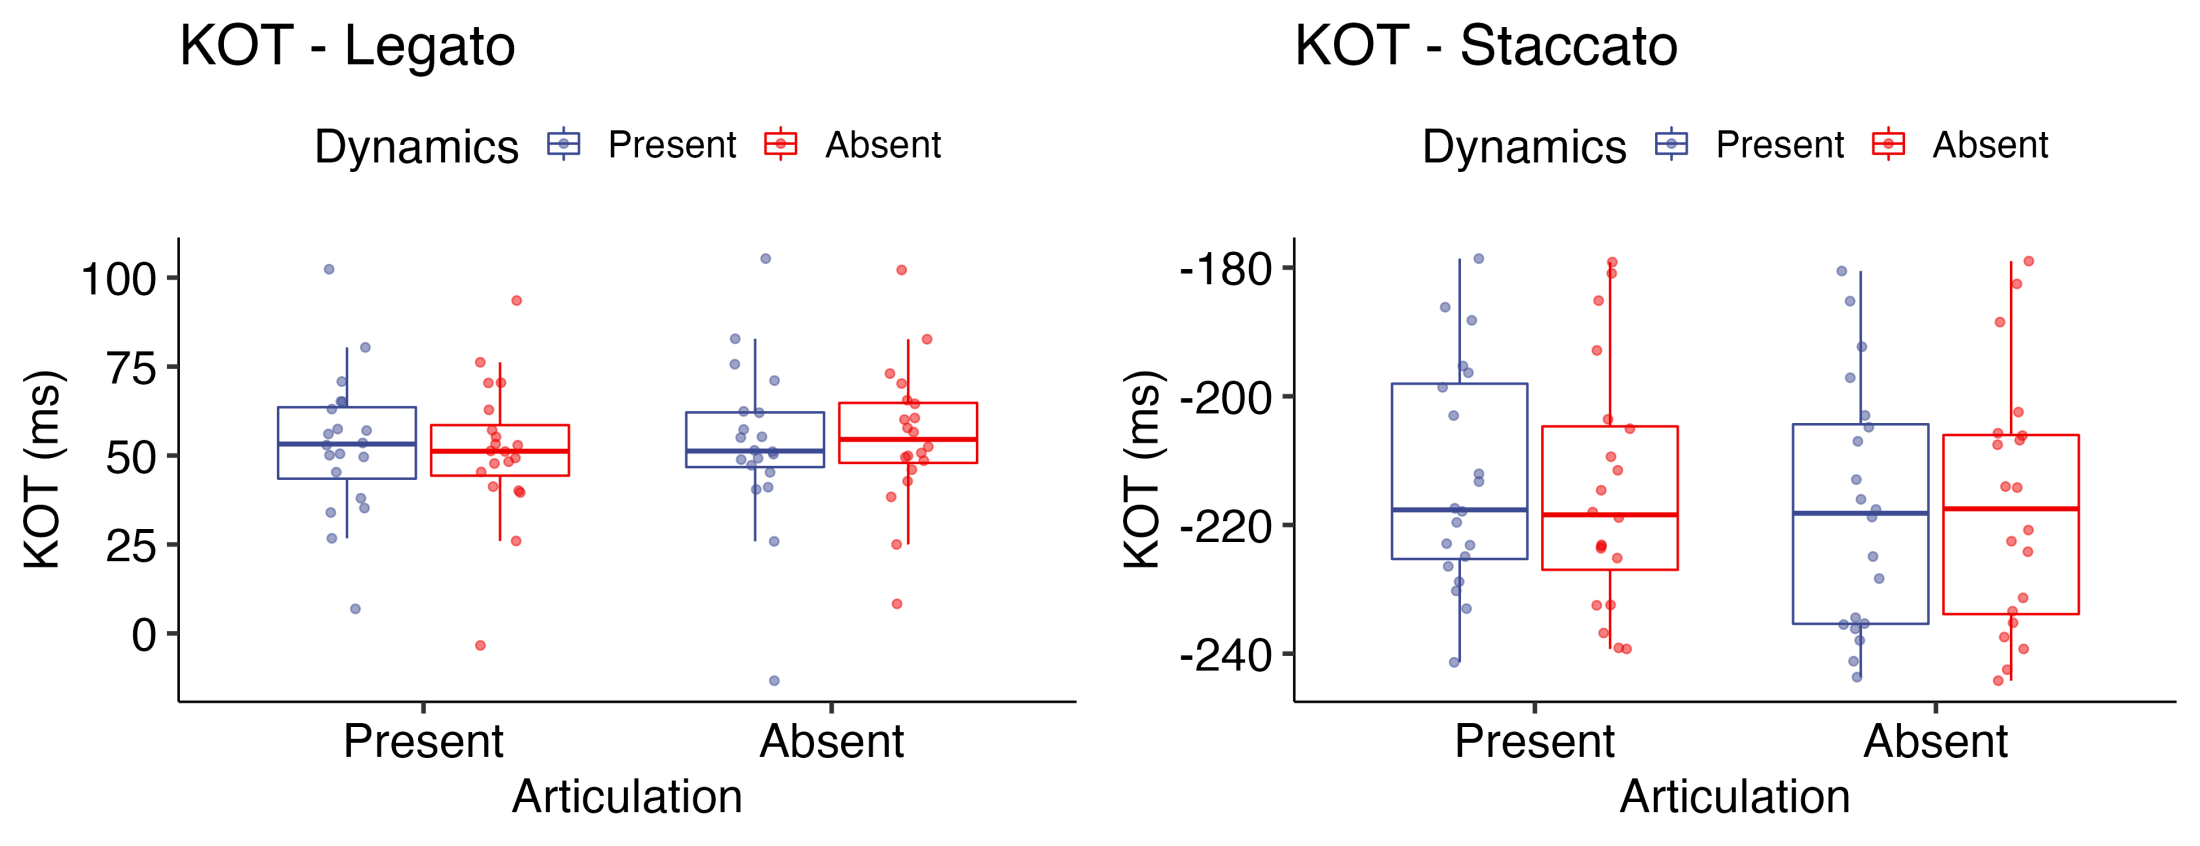
\includegraphics[width=1\linewidth]{manuscript_files/figure-latex/plot-kot-1-1} \caption{\label{fig:kot-1}KOT(ms) for each subcomponent; legato (left) and staccato (right). Each box indicates the IQR with the median, and whiskers extend to a maximum of 1.5 × IQR beyond the box.}\label{fig:plot-kot-1}
\end{figure}

\begin{figure}
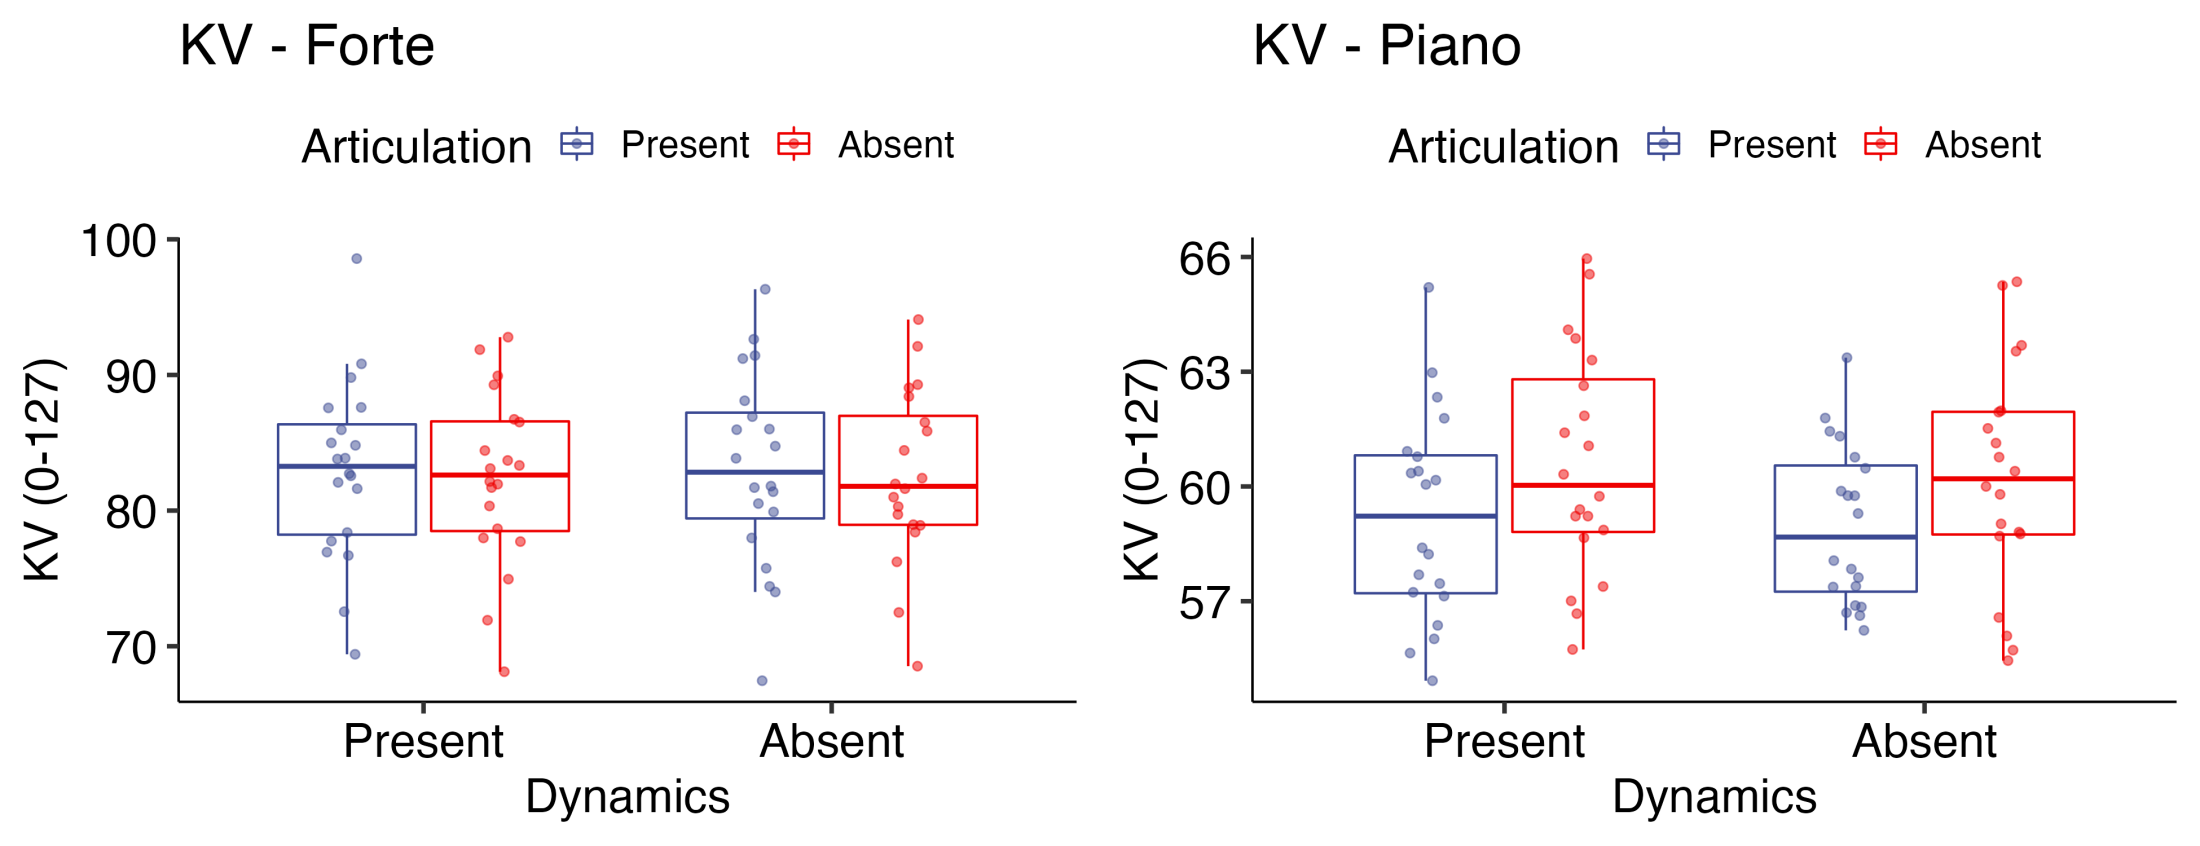
\includegraphics[width=1\linewidth]{manuscript_files/figure-latex/plot-vel-1-1} \caption{\label{fig:vel-1}KV (0-127) for each subcomponent; forte (left) and piano (right). Each box indicates the IQR with the median, and whiskers extend to a maximum of 1.5 × IQR beyond the box.}\label{fig:plot-vel-1}
\end{figure}

\begin{figure}
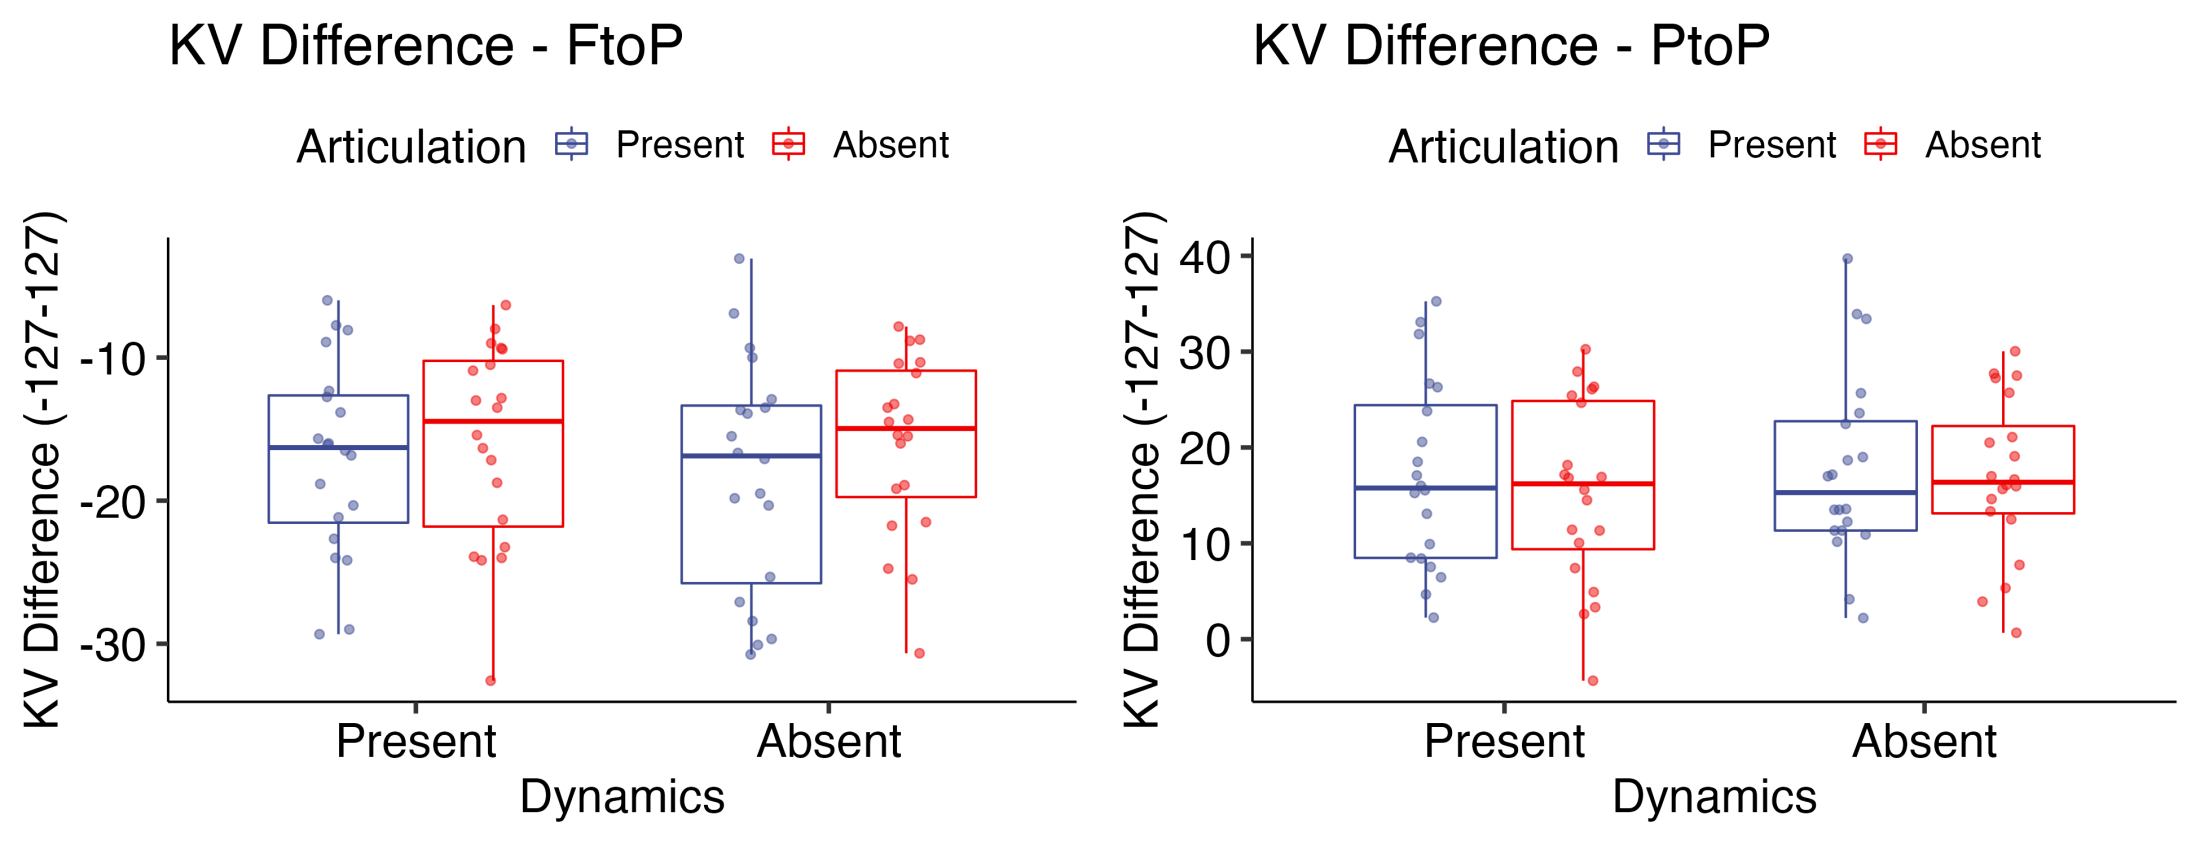
\includegraphics[width=1\linewidth]{manuscript_files/figure-latex/plot-vel-diff-1-1} \caption{\label{fig:vel-diff-1}KV Difference (-127-127) for each subcomponent; forte to piano (left) and piano to forte (right). Each box indicates the IQR with the median, and whiskers extend to a maximum of 1.5 × IQR beyond the box.}\label{fig:plot-vel-diff-1}
\end{figure}

\begin{figure}
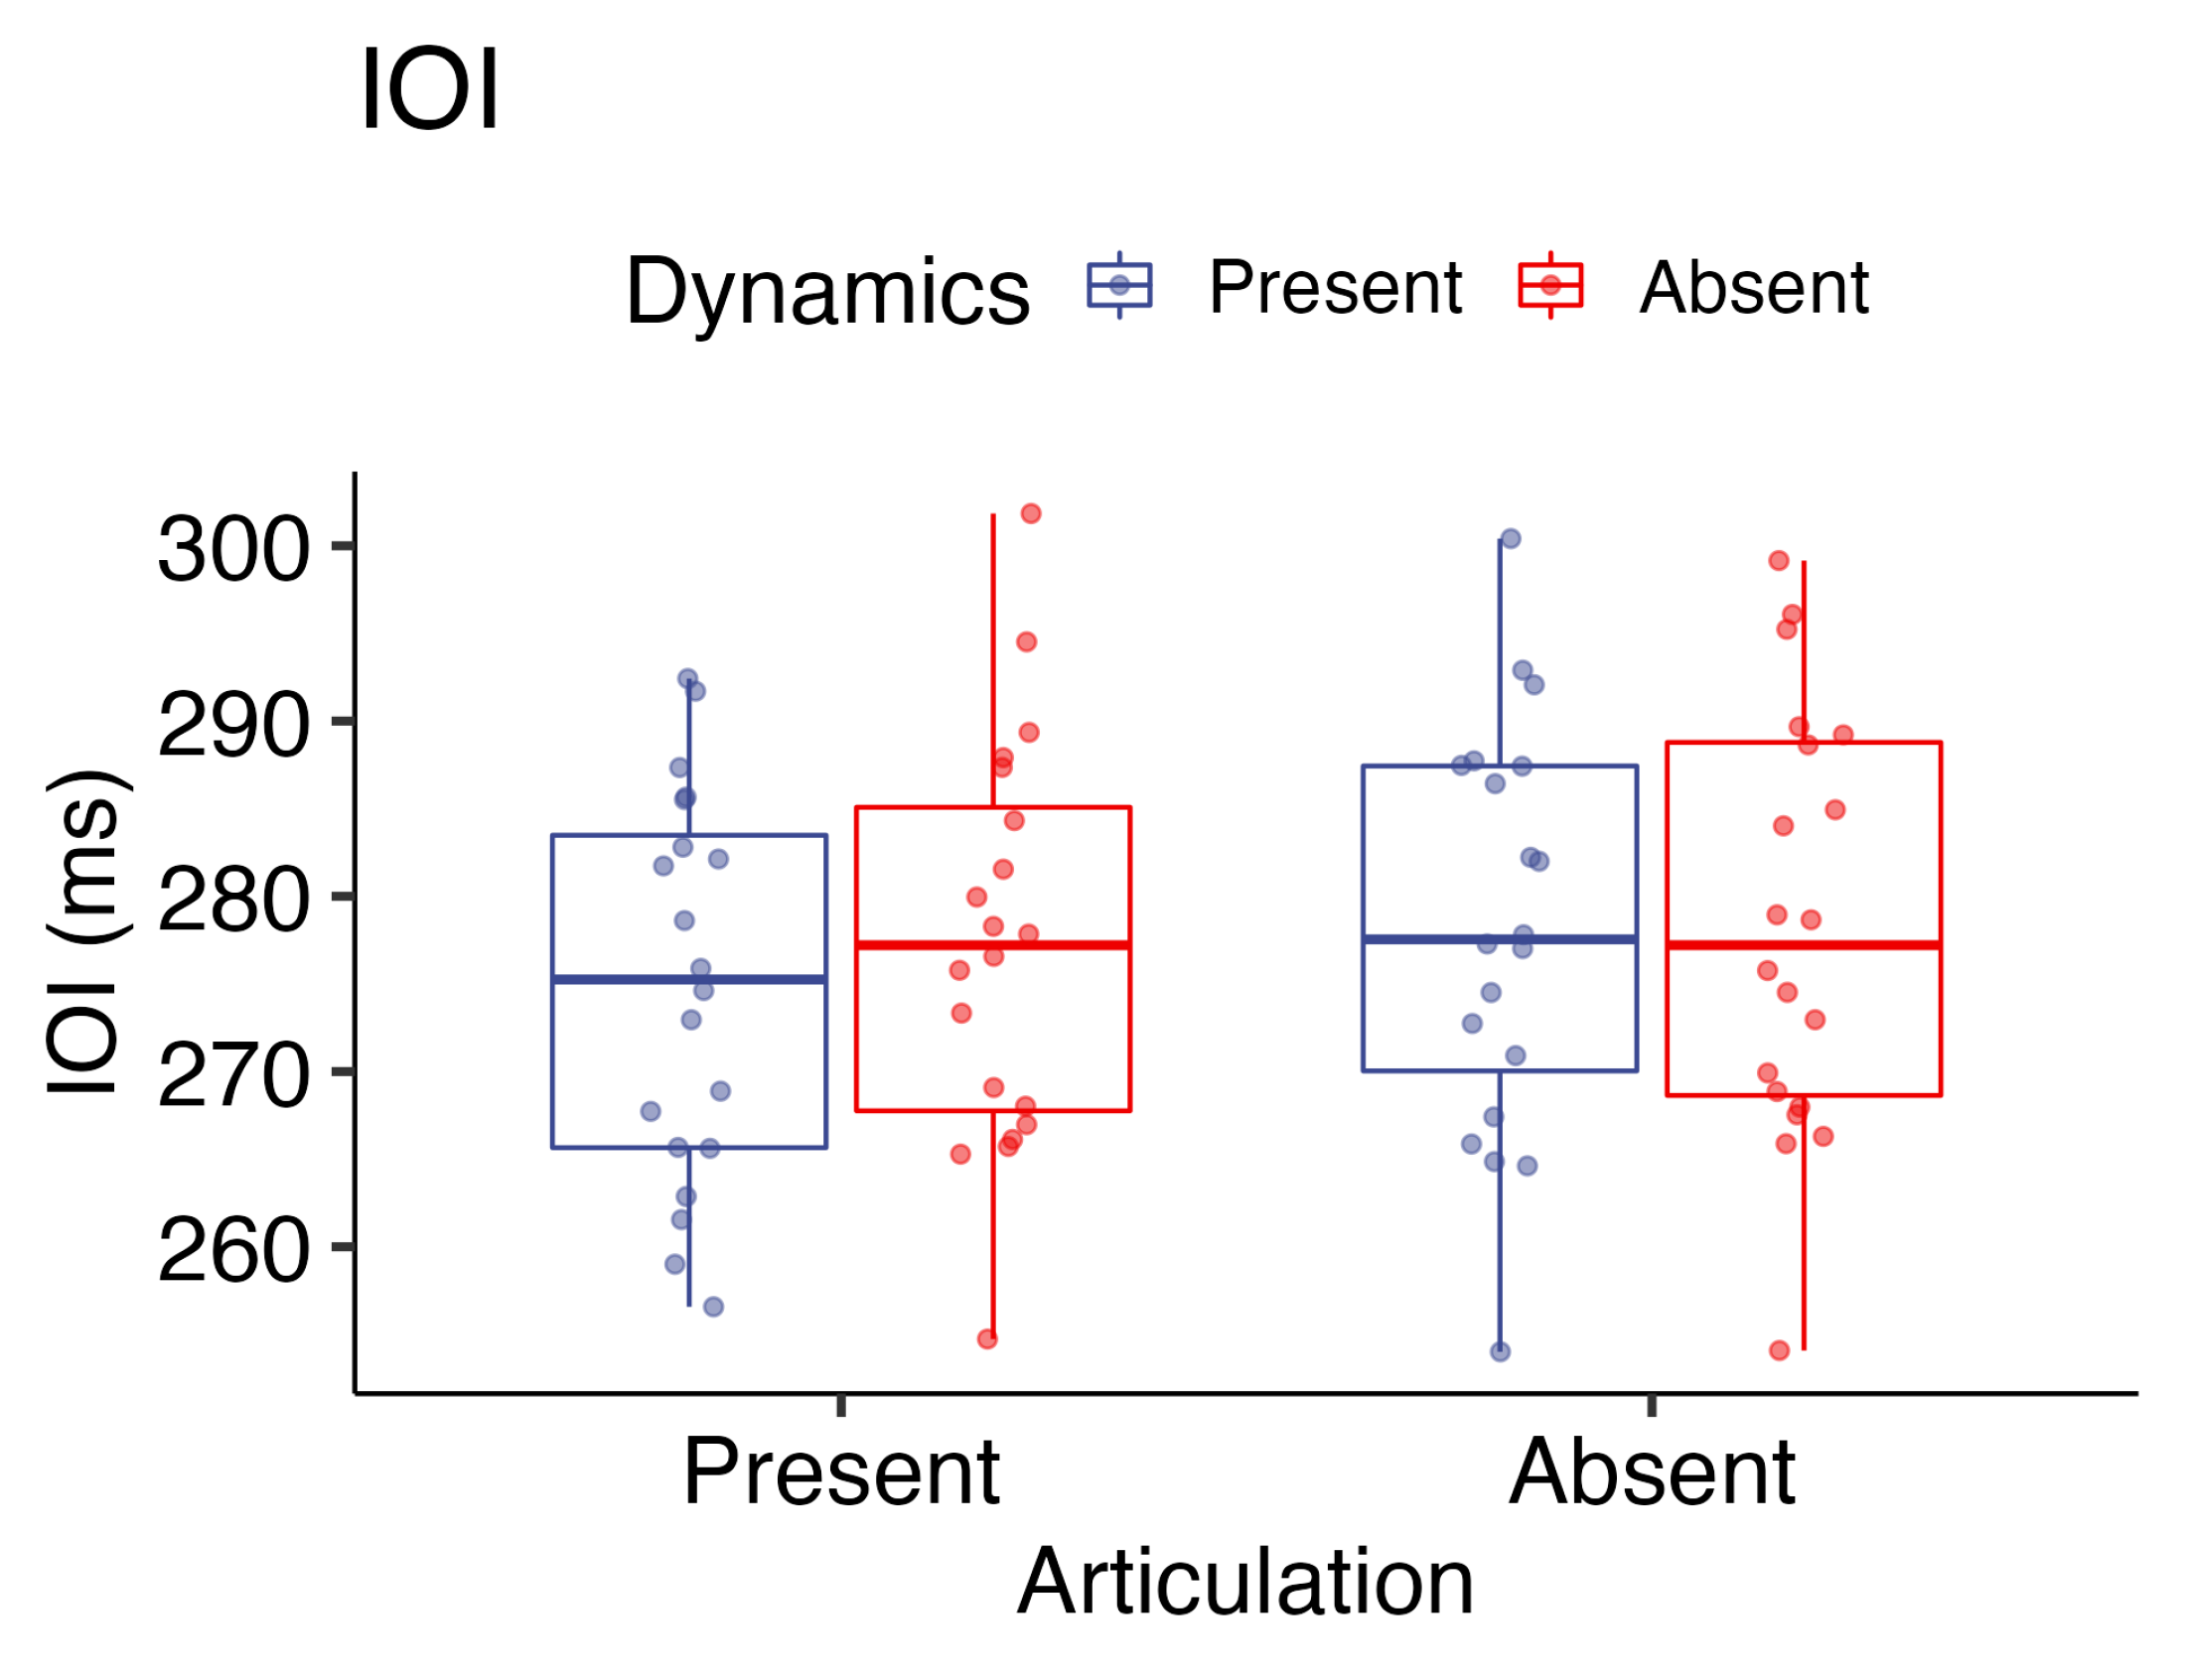
\includegraphics[width=1\linewidth]{manuscript_files/figure-latex/plot-ioi-1-1} \caption{\label{fig:ioi-1}IOIs (ms). A dashed line represents the tempo given by a metronome. Each box indicates the IQR with the median, and whiskers extend to a maximum of 1.5 × IQR beyond the box.}\label{fig:plot-ioi-1}
\end{figure}

\clearpage

\hypertarget{discussion}{%
\section{Discussion}\label{discussion}}

The present study investigated whether and how expert pianists adapt their performance depending on the displayed skills of novices whom they are intending to teach. We created artificial recordings to manipulate the implementation of two musical expressive techniques (i.e., articulation and dynamics) notated on the sheet music. The recordings where the two techniques were implemented were supposed to resemble the performances of students with good skills. The recordings where neither of the two techniques was implemented were supposed to resemble the performances of students with lower skills who had not yet learnt how to implement articulation and dynamics. The recordings where either of the two techniques was implemented but the other was missing were created to examine whether expert pianists could recognise a particular problem that students have (e.g., only articulation was missing) and adjust their performance accordingly (e.g., expert pianists should modulate their performance relevant to articulation, but not dynamics).

Expert pianists exaggerated legato and staccato when articulation was not implemented in the recordings. This is in line with our predictions that experts would exaggerate only the relevant aspects of the performance if a particular technique was missing in the recordings. However, we did not find significant results in terms of dynamics. Instead, we found that expert pianists produced softer piano when articulation was implemented in the recordings, indicating that participants exaggerated piano only when there was no problem with regard to articulation in the recordings. This may imply that participants prioritised the teaching of articulation over dynamics and did not modify two performance parameters at the same time. This is consistent with the findings in parental scaffolding where caregivers help infants acquire a complex action sequence by simplifying the sequential action into discrete sub-actions and adding complexity step by step (Zukow-Goldring \& Arbib, 2007).

The reason why expert pianists seemed to prioritise the teaching of articulation might be that articulation was more important for the specific piece we selected or that the piece itself naturally invited some implementation of articulation. In our previous study, we observed most participants implemented articulation (particularly legato) when they were asked to perform the piece even when neither articulation nor dynamics was notated on the sheet music. Therefore, it is possible that expert pianists were particularly sensitive to the lack of articulation in the recordings and trying to highlight it. Another possibility is that dynamics modulations in the recordings were too subtle to be noticed by participants and therefore they did not modulate the dynamics aspect of their performance.

We also found that expert pianists did not modulate their tempo (IOIs) depending on the displayed skill level of students. Also compared with the tempo of the baseline performance (see \emph{Supplementary Material}), they did not change the tempo in the teaching context. These findings indicated that tempo was not employed specifically in teaching, likely because tempo itself was not relevant to either articulation or dynamics. Although slower demonstration is generally considered to be used for teaching (Brand et al., 2002; McEllin et al., 2017; Schaik, Meyer, Ham, \& Hunnius, 2019), in music performance, it may not be an effective strategy to perform slowly as changing the tempo might give another interpretation to the music.

There are possibilities that it may be difficult in general for experts to flexibly adjust to different action parameters while teaching or they might have chosen to focus on the most salient parameters or the ones that they find most relevant. For example, when teaching dance, it is considered that good teachers identify and build the basic knowledge and skills first and then add complexity progressively from the basic foundation (Mainwaring \& Krasnow, 2010). When teaching social dance, a teacher started with a basic step as the hustle and then moved onto more complex steps progressively like the waltz and the cha cha (Lobel, 2021). Karl Leimer, a German music teacher and pianist, wrote in his booked that students should perform with legato at first in finger exercises such as the playing of scales (Gieseking \& Leimer, 1972). In both dance and music examples, the ultimate goal of skill acquisition is that students are able to use multiple techniques flexibly while performing. However, it seems that students need to build complex skills progressively based on the basics during the learning process. Therefore, identifying and focusing on the most relevant problem for each student may be more effective to facilitate skill acquisition.

One of the limitations of the current study is that participants may not have had a clear idea about what to teach because they did not have a normative ideal performance in mind. As some participants reported that ``(students had) very different interpretations of the melody'' or ``all kids played rhythmically correct'' in the questionnaire, it is plausible that the lack of articulation and/or dynamics might not have been perceived as errors. One solution would be to provide a model performance where both articulation and dynamics are implemented and ask participants to listen to it first so that they can detect errors by comparing each recording with the model performance.

The reason why participants considered different recording variations as interpretations rather than errors might stem from the fact that all the recordings did not include any pitch errors and were performed with a stable tempo. This was to make sure that only articulation and dynamics features of the recordings varied. However, some of the recordings might not have sounded as if unskillful students were playing. In order to create more realistic novice performances, it might be useful to add some jitters to the tempo of the recordings we created, or to ask beginner pianists to play the piece and extract the temporal features of their performances.

Experiments which investigated dynamic interactions between experts and novices have been done with the physical presence of both an expert and a novice in the same place (Fukuyama et al., 2015; Okazaki, Muraoka, \& Osu, 2019; Zukow-Goldring \& Arbib, 2007). In the current experiment, expert pianists had only access to their imaginary students and needed to perform in the absence of actual students. Future research should investigate how expert pianists and novices dynamically interact in a situation where they can communicate in real-time and examine how the performance of expert pianists and that of novices are related to each other.

\clearpage

\hypertarget{references}{%
\section{References}\label{references}}

\begingroup
\setlength{\parindent}{-0in}
\setlength{\leftskip}{0in}

\hypertarget{refs}{}
\begin{CSLReferences}{1}{0}
\leavevmode\vadjust pre{\hypertarget{ref-brand_2002}{}}%
Brand, R. J., Baldwin, D. A., \& Ashburn, L. A. (2002). Evidence for {``motionese''}: Modifications in mothers' infant-directed action. \emph{Developmental Science}, \emph{5}(1), 72--83. \url{https://doi.org/10.1111/1467-7687.00211}

\leavevmode\vadjust pre{\hypertarget{ref-byrne_2011}{}}%
Byrne, R. W., \& Rapaport, L. G. (2011). What are we learning from teaching? \emph{Animal Behaviour}, \emph{82}(5), 1207--1211. \url{https://doi.org/10.1016/j.anbehav.2011.08.018}

\leavevmode\vadjust pre{\hypertarget{ref-cancino-chacon_2018}{}}%
Cancino-Chacón, C. E., Grachten, M., Goebl, W., \& Widmer, G. (2018). Computational {Models} of {Expressive Music Performance}: {A Comprehensive} and {Critical Review}. \emph{Frontiers in Digital Humanities}, \emph{5}.

\leavevmode\vadjust pre{\hypertarget{ref-fukuyama_2015}{}}%
Fukuyama, H., Qin, S., Kanakogi, Y., Nagai, Y., Asada, M., \& Myowa-Yamakoshi, M. (2015). Infant's action skill dynamically modulates parental action demonstration in the dyadic interaction. \emph{Developmental Science}, \emph{18}(6), 1006--1013. \url{https://doi.org/10.1111/desc.12270}

\leavevmode\vadjust pre{\hypertarget{ref-gieseking_1972}{}}%
Gieseking, W., \& Leimer, K. (1972). \emph{Piano {Technique}}. {Dover Publications}.

\leavevmode\vadjust pre{\hypertarget{ref-lobel_2021}{}}%
Lobel, E. E. (2021). A {Model} for {Integrating Social} and {Creative Dance Forms} in a {Dance Education Course}. \emph{Journal of Dance Education}, \emph{21}(1), 44--47. \url{https://doi.org/10.1080/15290824.2020.1732984}

\leavevmode\vadjust pre{\hypertarget{ref-mainwaring_2010}{}}%
Mainwaring, L. M., \& Krasnow, D. H. (2010). Teaching the {Dance Class}: {Strategies} to {Enhance Skill Acquisition}, {Mastery} and {Positive Self-Image}. \emph{Journal of Dance Education}, \emph{10}(1), 14--21. \url{https://doi.org/10.1080/15290824.2010.10387153}

\leavevmode\vadjust pre{\hypertarget{ref-mcellin_2017}{}}%
McEllin, L., Knoblich, G., \& Sebanz, N. (2017). Distinct kinematic markers of demonstration and joint action coordination? {Evidence} from virtual xylophone playing. \emph{Journal of Experimental Psychology: Human Perception and Performance}, \emph{44}(6), 885. \url{https://doi.org/10.1037/xhp0000505}

\leavevmode\vadjust pre{\hypertarget{ref-mermelshtine_2017}{}}%
Mermelshtine, R. (2017). Parent\textendash child learning interactions: {A} review of the literature on scaffolding. \emph{British Journal of Educational Psychology}, \emph{87}(2), 241--254. \url{https://doi.org/10.1111/bjep.12147}

\leavevmode\vadjust pre{\hypertarget{ref-okazaki_2019}{}}%
Okazaki, S., Muraoka, Y., \& Osu, R. (2019). Teacher-learner interaction quantifies scaffolding behaviour in imitation learning. \emph{Scientific Reports}, \emph{9}(1), 1--13. \url{https://doi.org/10.1038/s41598-019-44049-x}

\leavevmode\vadjust pre{\hypertarget{ref-pezzulo_2019}{}}%
Pezzulo, G., Donnarumma, F., Dindo, H., D'Ausilio, A., Konvalinka, I., \& Castelfranchi, C. (2019). The body talks: {Sensorimotor} communication and its brain and kinematic signatures. \emph{Physics of Life Reviews}, \emph{28}, 1--21. \url{https://doi.org/10.1016/j.plrev.2018.06.014}

\leavevmode\vadjust pre{\hypertarget{ref-schaik_2019}{}}%
Schaik, J. E. van, Meyer, M., Ham, C. R. van, \& Hunnius, S. (2019). Motion tracking of parents' infant- versus adult-directed actions reveals general and action-specific modulations. \emph{Developmental Science}, \emph{0}(0), e12869. \url{https://doi.org/10.1111/desc.12869}

\leavevmode\vadjust pre{\hypertarget{ref-tominaga_2022}{}}%
Tominaga, A., Knoblich, G., \& Sebanz, N. (2022). Expert pianists make specific exaggerations for teaching. \emph{Scientific Reports}, \emph{12}(1), 21296. \url{https://doi.org/10.1038/s41598-022-25711-3}

\leavevmode\vadjust pre{\hypertarget{ref-ugur_2015}{}}%
Ugur, E., Nagai, Y., Celikkanat, H., \& Oztop, E. (2015). Parental scaffolding as a bootstrapping mechanism for learning grasp affordances and imitation skills. \emph{Robotica}, \emph{33}(5), 1163--1180. \url{https://doi.org/10.1017/S0263574714002148}

\leavevmode\vadjust pre{\hypertarget{ref-wood_1975}{}}%
Wood, D., \& Middleton, D. (1975). A {Study} of {Assisted Problem-Solving}. \emph{British Journal of Psychology}, \emph{66}(2), 181--191. \url{https://doi.org/10.1111/j.2044-8295.1975.tb01454.x}

\leavevmode\vadjust pre{\hypertarget{ref-zukow-goldring_2007}{}}%
Zukow-Goldring, P., \& Arbib, M. A. (2007). Affordances, effectivities, and assisted imitation: {Caregivers} and the directing of attention. \emph{Neurocomputing}, \emph{70}(13), 2181--2193. \url{https://doi.org/10.1016/j.neucom.2006.02.029}

\end{CSLReferences}

\endgroup

\hypertarget{acknowledgement}{%
\section{Acknowledgement}\label{acknowledgement}}

This research was supported by the European Research Council under the European Union's Seventh Framework Program (FP7/2007--2013)/ERC Grant agreement no. 609819, SOMICS, and by ERC Grant agreement no. 616072, JAXPERTISE. We thank Candasch Acar for his help with data collection.

\clearpage

\hypertarget{supplementary-material}{%
\section{Supplementary Material}\label{supplementary-material}}

\hypertarget{artificial-recordings}{%
\subsection{1. Artificial recordings}\label{artificial-recordings}}

Artificial recordings were generated from performance data that we obtained in our previous study (Tominaga et al., 2022). We used the data from Experiment 2. In Experiment 2, participants were asked to memorise one piece of music (\emph{Fig 5} (A), Tominaga et al. (2022)) without any expressive notation before coming to the experiment. First, we asked participants to perform the memorised piece before starting the experiment to measure their baseline performance. After measuring the baseline performance, participants were asked to perform the piece with either articulation (\emph{Fig 5} (B), Tominaga et al. (2022)) or dynamics (\emph{Fig 5} (C), Tominaga et al. (2022)) in two conditions (teaching vs.~performing). Here, we only used the data from the performing condition to make sure that the performances that we used did not have any particular modulations because of teaching intentions. Therefore, there were two types of performance data (articulation performance: performances played with notated articulation, dynamics performance: performances played with notated dynamics). We obtained 31 valid performances (i.g., performances without pitch errors) as baseline performances, 137 valid performances as articulation performances and 139 valid performances as dynamics performances.

\hypertarget{procedure-1}{%
\subsubsection{1. Procedure}\label{procedure-1}}

We aimed to generate four types of recordings and each type (i.e., both, art only, dyn only, none) had four instances (see \emph{Apparatus and stimuli}) by using the performance data from Tominaga et al. (2022). First, 16 instances for each type were generated. Second, for each type, we chose the four best instances, which exhibited the characteristic of each type well.

\hypertarget{generation-of-16-instances-per-each-type}{%
\subsubsection{2. Generation of 16 instances per each type}\label{generation-of-16-instances-per-each-type}}

In order to create recordings, we needed information about 1) the pitch order, 2) when each note was pressed (related to tempo), 3) when each note was released (related to articulation) and 4) how fast each note was hit (related to dynamics). Pitch information was already determined and the same for all structures because of the sheet music (\emph{Fig \ref{fig:stim}}).

First, we created 16 basic structures of recordings from the baseline performances. To determine the temporal feature of each structure (i.e., when each key was pressed), three performances out of the 31 valid baseline performances were randomly selected and interonset intervals (IOIs) of the three performances were averaged. Due to the size of the dataset (i.e., 31 performances), some baseline performances were used twice. We made sure that the identical performance was not selected within each random selection (i.e., each selection consisted of three different performances). Thus, we created 16 basic structures for tempi.

Next, we were going to follow the same procedure to determine the sound duration (i.e., when each key was released) of each note (related to articulation) and the key velocity profile (i.e., how fast each key was hit) of each note (related to dynamics). For the sound duration, however, we found that most participants implemented articulation (particularly legato) even in their baseline performances, where they should not implement any particular articulation or dynamics. Therefore, we decided to use the data from only two participants who did not show such tendencies. We obtained four performances from the two participants and used these four performances four times each without performing any averaging so as to have 16 instances in total. For the key velocity profiles, we followed the same procedure as we determined tempi and three performances out of the 31 valid baseline performances were randomly selected and the key velocity profiles of the three performances were averaged. This is how we created 16 instances for three performance features (i.e., tempo, articulation and dynamics). We generated the 16 recordings where neither articulation nor dynamics was implemented (i.e., none) by combining the three performance features made from the baseline performances.

In order to have other three types of recordings (i.e., both, art only, dyn only), we needed to create 16 instances for the sound duration when articulation was implemented and 16 instances for the key velocity profiles when dynamics was implemented. We followed the same procedure as we did to generate none recordings but we used articulation performances (not baseline performances) for the sound duration and dynamics performances (not baseline performances) for the key velocity profiles. To create art only recordings,

\hypertarget{selection-of-four-instances-per-type}{%
\subsubsection{3. Selection of four instances per type}\label{selection-of-four-instances-per-type}}

After we generated 16 recordings for each type, we asked 3 musician raters including the first author to listen to each generated recording and rate to what extent each expression was implemented between 0 (not at all) and 5 (fully). Based on these ratings, we selected four recordings for each type.

\hypertarget{comparison-with-baseline-performance}{%
\subsection{2. Comparison with baseline performance}\label{comparison-with-baseline-performance}}

To recall the instruction for the baseline performance, we asked participants to perform the piece expressively with their interpretation and to do their best as a performer. By comparing with the baseline performance, we can investigate how pedagogical intentions influence participants' performances.

\hypertarget{kot-1}{%
\subsection{KOT}\label{kot-1}}

We compared the baseline performance with the performances in response to recordings where dynamics was implemented to examine whether participants performed differently depending on whether articulation was implemented or not in each recording. We categorised performances into three groups (baseline, both (i.e., articulation-present, dynamics-present), dynamics-only (i.e., articulation-absent, dynamics-present)) and treated them as a factor Category.

\hypertarget{legato-1}{%
\subsubsection{Legato}\label{legato-1}}

There was a significant main effect of Category (\emph{F}(1.45, 27.53) = 11.82, \emph{p} \textless{} 0.001, \(\eta_G^2\) = 0.060; Greenhouse-Geisser corrected). Post-hoc comparisons based on the estimated marginal means with Tukey adjustment showed that there were differences between baseline and the other two categories (baseline and both: \emph{p} \textless{} .001, baseline and dynamics-only: \emph{p} = .008), suggesting that participants produced longer legato when they had the intention to teach (\emph{Fig \ref{fig:kot-2}}, left).

\hypertarget{staccato-1}{%
\subsubsection{Staccato}\label{staccato-1}}

There was no significant main effect of Category (\emph{F}(1.12, 21.28) = 0.75, \emph{p} = 0.41, \(\eta_G^2\) = 0.011; Greenhouse-Geisser corrected), suggesting that participants did not play staccato differently depending on whether they had the intention to teach (\emph{Fig \ref{fig:kot-2}}, right).

\hypertarget{kv-1}{%
\subsection{KV}\label{kv-1}}

We compared the baseline performance with the performances in response to recordings where articulation was implemented to examine whether participants performed differently depending on whether dynamics was implemented or not in each recording. We categorised performances into three groups (baseline, both (i.e., articulation-present, dynamics-present), articulation-only (i.e., articulation-present, dynamics-absent)) and treated them as a factor Category.

\hypertarget{forte-1}{%
\subsubsection{Forte}\label{forte-1}}

There was no significant main effect of Category (\emph{F}(1.59, 30.18) = 1.43, \emph{p} = 0.25, \(\eta_G^2\) = 0.004; Greenhouse-Geisser corrected), suggesting that participants did not play forte differently depending on whether they had the intention to teach (\emph{Fig \ref{fig:vel-2}}, left).

\hypertarget{piano-1}{%
\subsubsection{Piano}\label{piano-1}}

There was a significant main effect of Category (\emph{F}(1.79, 34.09) = 5.68, \emph{p} = 0.009, \(\eta_G^2\) = 0.072; Greenhouse-Geisser corrected). Post-hoc comparisons based on the estimated marginal means with Tukey adjustment showed that there were differences between baseline and the other two categories (baseline and both: \emph{p} = .05, baseline and articulation-only: \emph{p} = .03), suggesting that participants produced softer piano when they had the intention to teach (\emph{Fig \ref{fig:vel-2}}, right).

\hypertarget{kv-difference-1}{%
\subsection{KV Difference}\label{kv-difference-1}}

We compared the baseline performance with the performances in response to recordings where articulation was implemented to examine whether participants performed differently depending on whether dynamics was implemented or not in each recording. We categorised performances into three groups (baseline, both (i.e., articulation-present, dynamics-present), articulation-only (i.e., articulation-present, dynamics-absent)) and treated them as a factor Category.

\hypertarget{forte-to-piano-1}{%
\subsubsection{Forte to Piano}\label{forte-to-piano-1}}

There was no significant main effect of Category (\emph{F}(1.53, 29.15) = 1.73, \emph{p} = 0.20, \(\eta_G^2\) = 0.014; Greenhouse-Geisser corrected).

\hypertarget{piano-to-forte-1}{%
\subsubsection{Piano to Forte}\label{piano-to-forte-1}}

There was no significant main effect of Category (\emph{F}(1.28, 24.39) = 2.27, \emph{p} = 0.14, \(\eta_G^2\) = 0.013; Greenhouse-Geisser corrected).

These results indicated that participants did not make dynamics contrast between forte and piano differently depending on whether they had the intention to teach (\emph{Fig \ref{fig:vel-diff-2}}).

\hypertarget{iois-1}{%
\subsection{IOIs}\label{iois-1}}

We compared the baseline performance with the performances in response to recordings where either both articulation and dynamics were implemented or neither of them was implemented. The reason for choosing this comparison was that we wanted to test whether having the intention to teach would lead to slower performances, either regardless of the learner's skill or especially when skills appeared to be lacking. We categorised performances into three groups (baseline, both, none) and treated them as a factor Category.

There was no significant main effect of Category (\emph{F}(1.11, 21.18) = 0.58, \emph{p} = 0.47, \(\eta_G^2\) = 0.012; Greenhouse-Geisser corrected), suggesting that participants kept the same tempo regardless of whether they had the intention to teach (\emph{Fig \ref{fig:ioi-2}}).

\begin{figure}
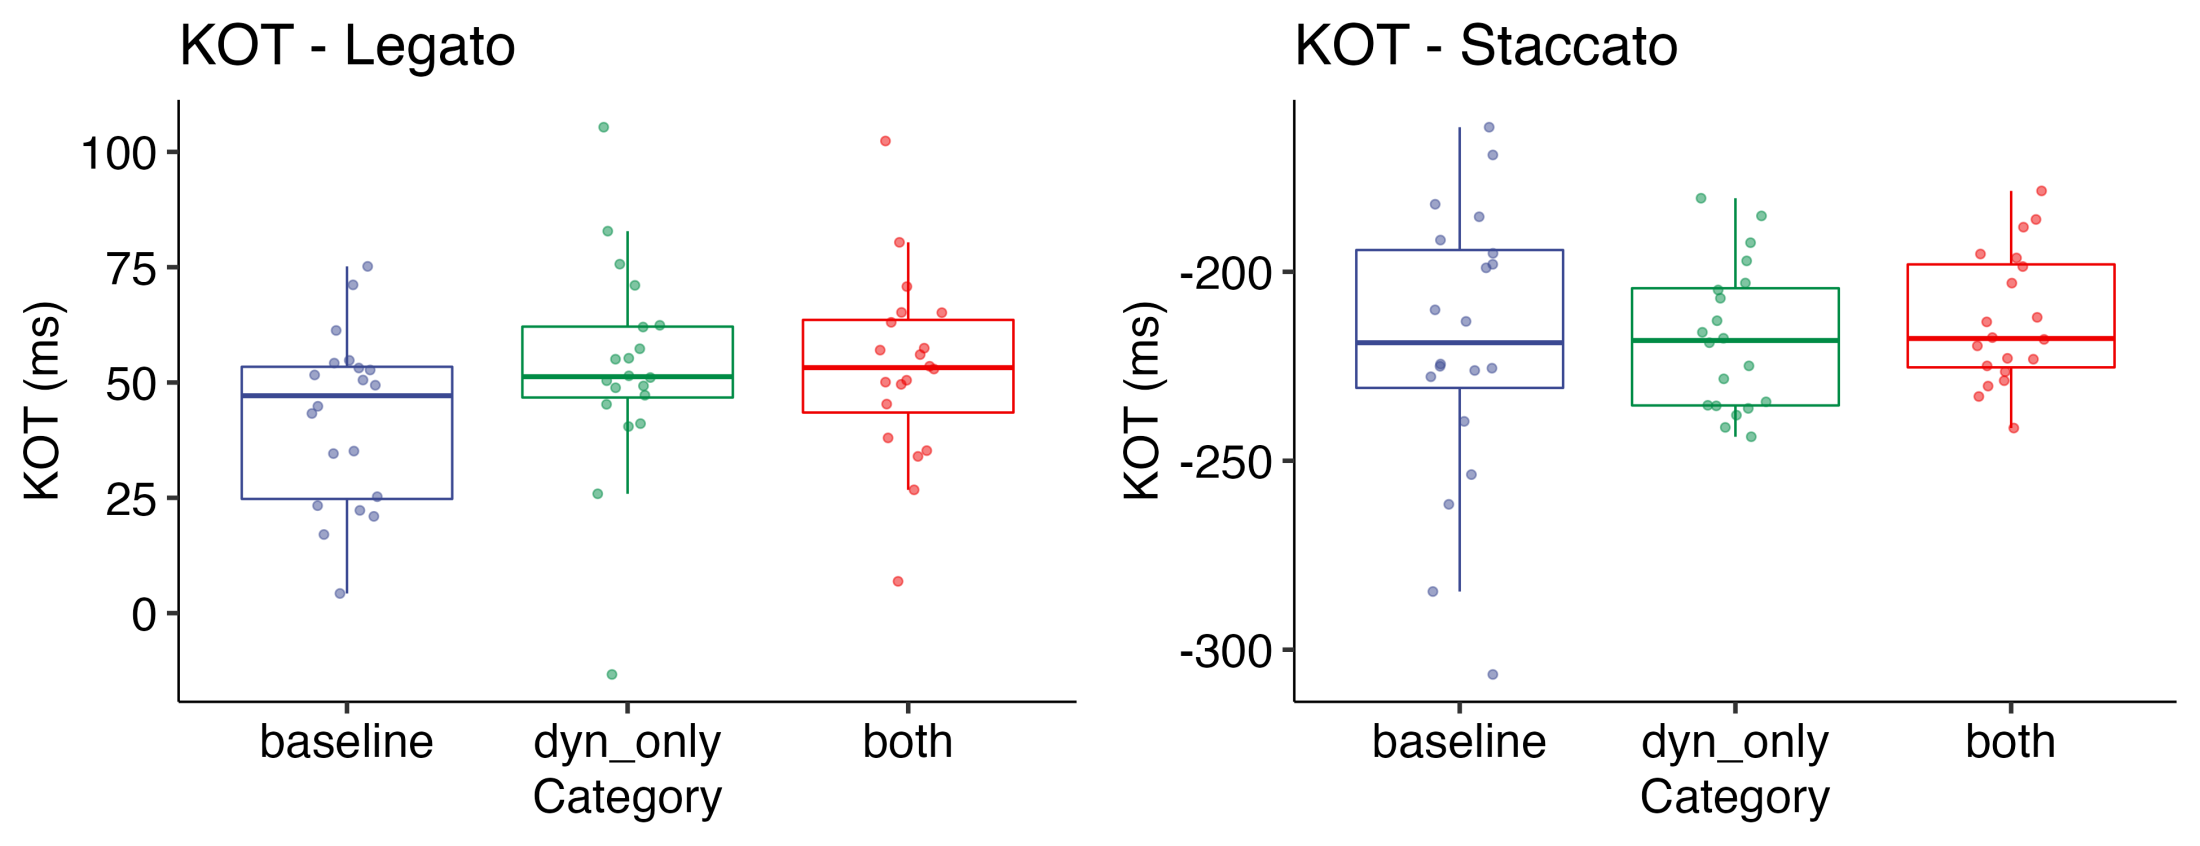
\includegraphics[width=1\linewidth]{manuscript_files/figure-latex/plot-kot-2-1} \caption{\label{fig:kot-2}Comparison with the baseline performance in terms of KOT(ms) for each subcomponent; legato (left) and staccato (right). Each box indicates the IQR with the median, and whiskers extend to a maximum of 1.5 × IQR beyond the box.}\label{fig:plot-kot-2}
\end{figure}

\begin{figure}
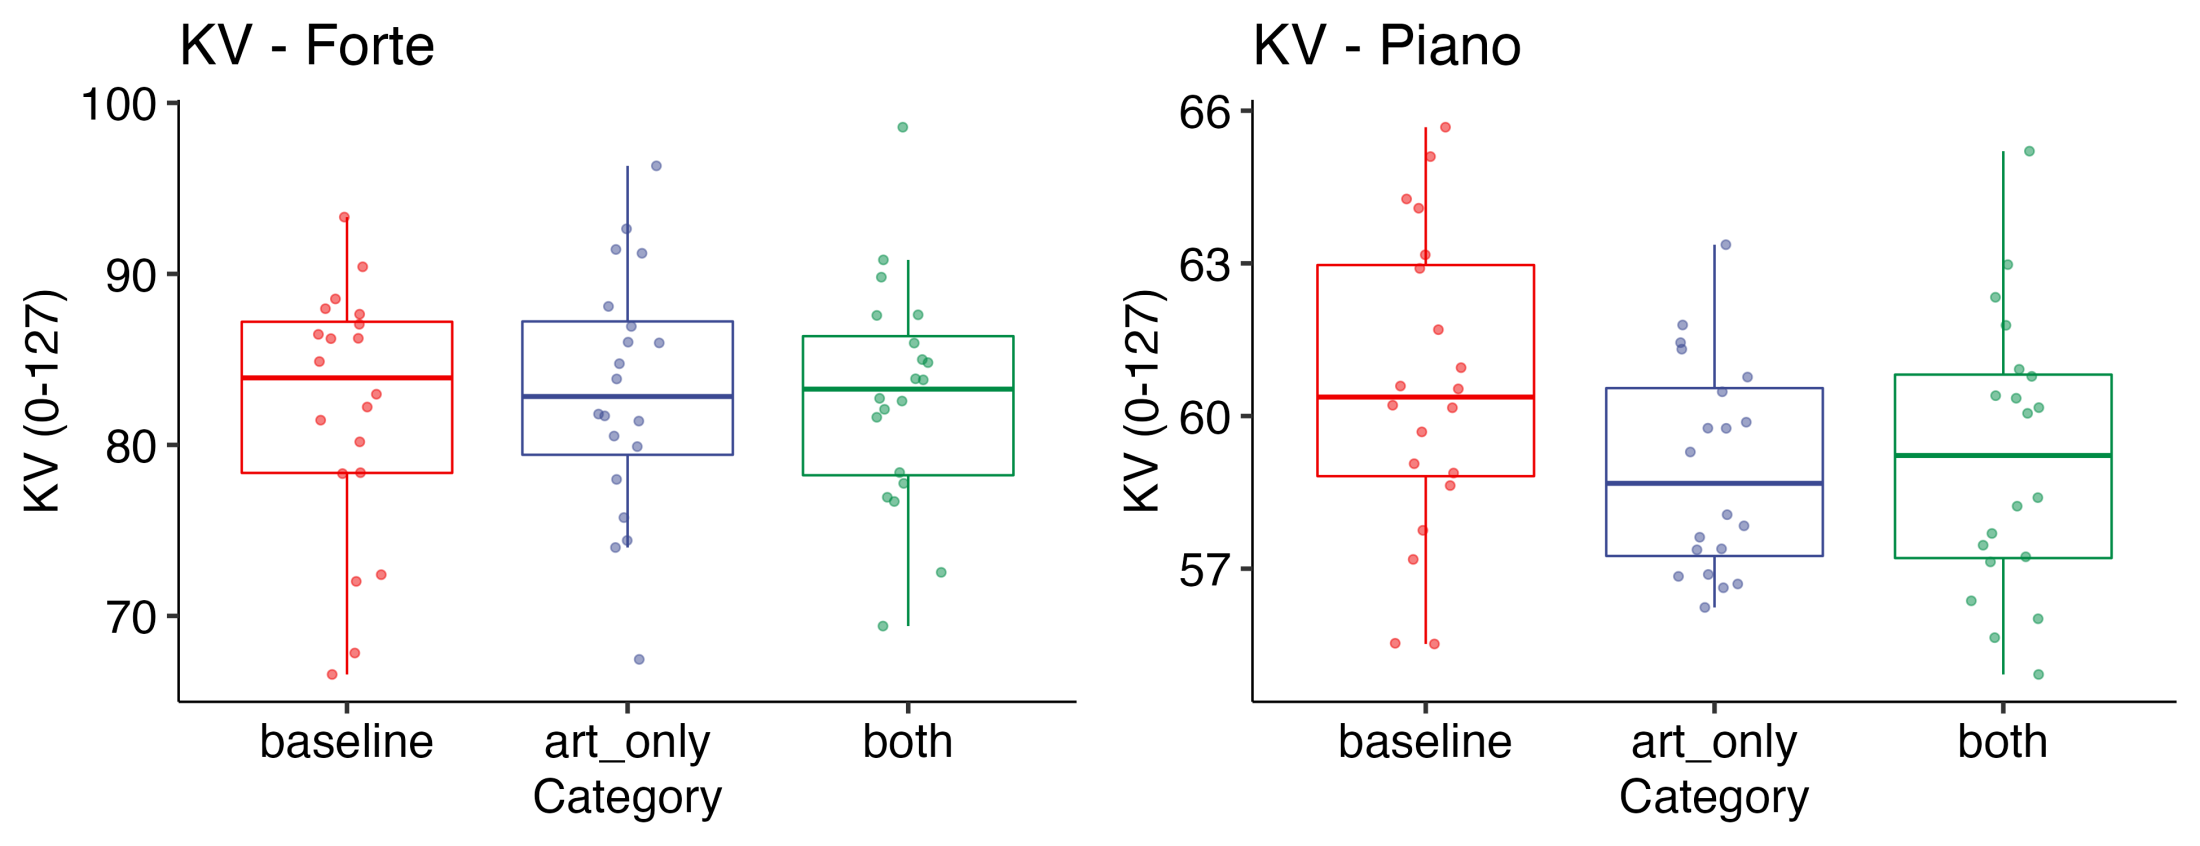
\includegraphics[width=1\linewidth]{manuscript_files/figure-latex/plot-vel-2-1} \caption{\label{fig:vel-2}Comparison with the baseline performance in terms of KV (0-127) for each subcomponent; forte (left) and piano (right). Each box indicates the IQR with the median, and whiskers extend to a maximum of 1.5 × IQR beyond the box.}\label{fig:plot-vel-2}
\end{figure}

\begin{figure}
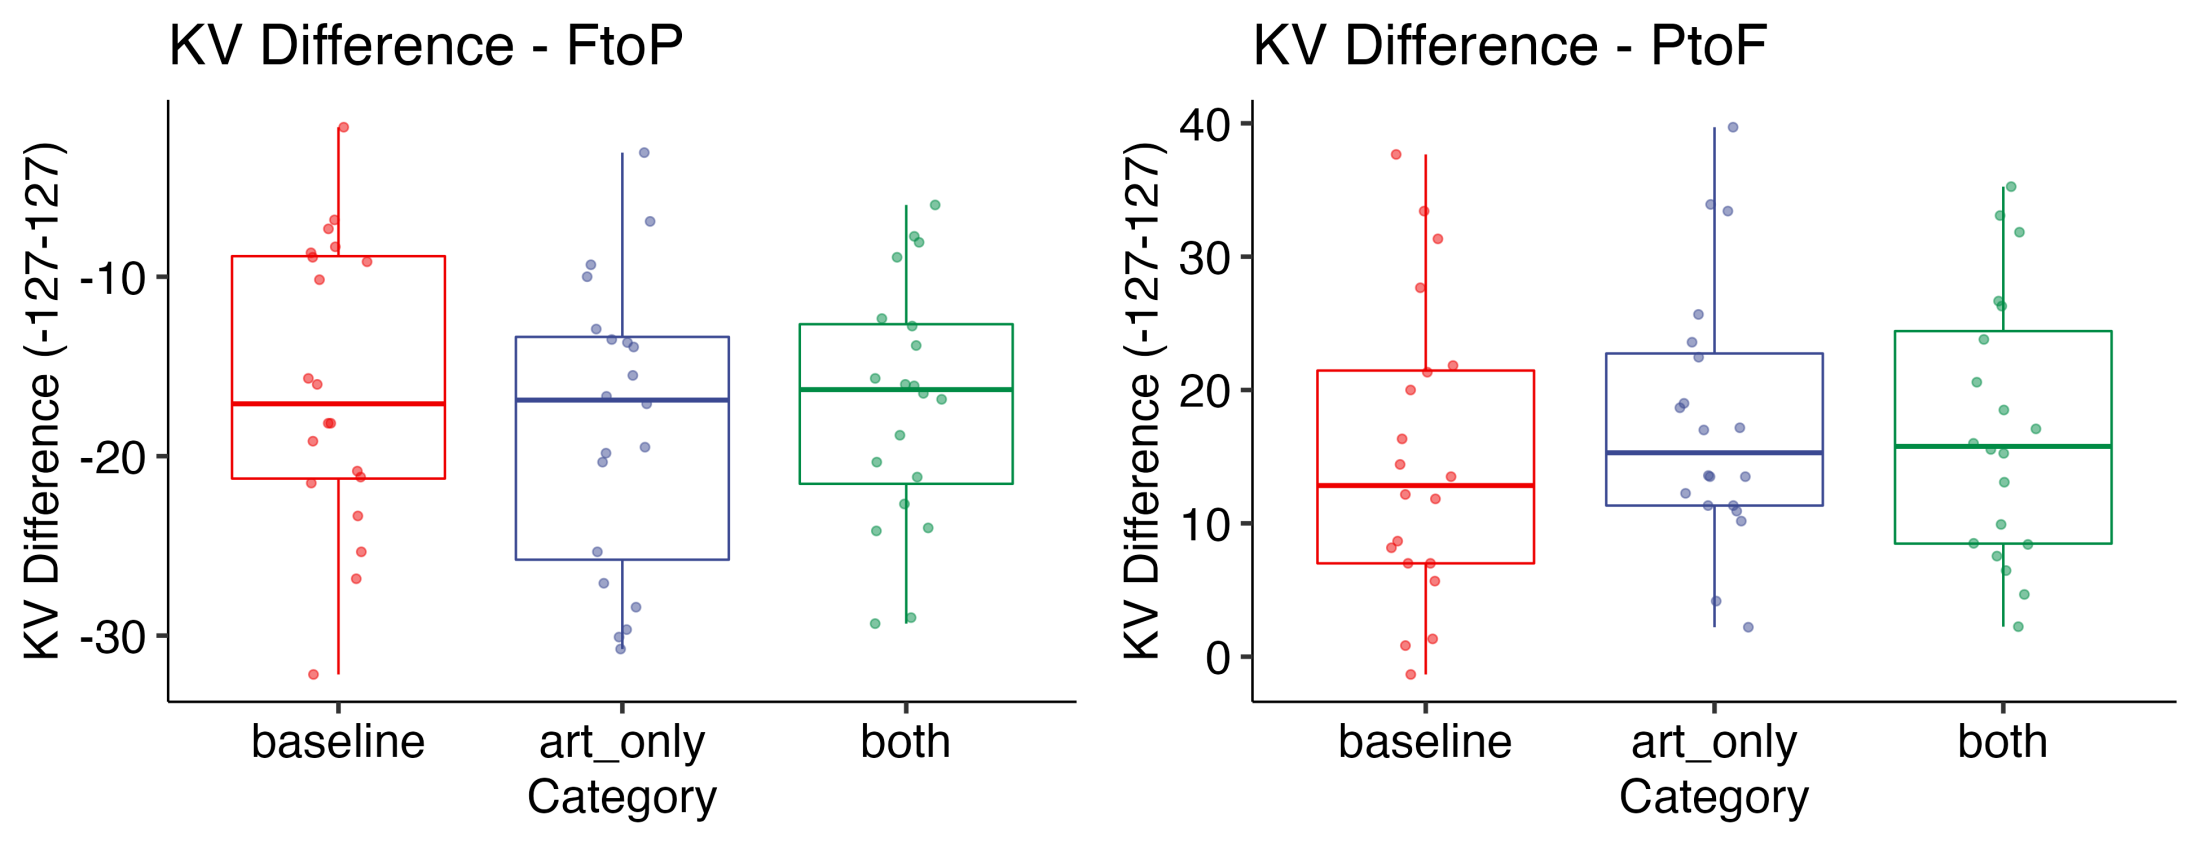
\includegraphics[width=1\linewidth]{manuscript_files/figure-latex/plot-vel-diff-2-1} \caption{\label{fig:vel-diff-2}Comparison with the baseline performance in terms of KV Difference (-127-127) for each subcomponent; forte to piano (left) and piano to forte (right). Each box indicates the IQR with the median, and whiskers extend to a maximum of 1.5 × IQR beyond the box.}\label{fig:plot-vel-diff-2}
\end{figure}

\begin{figure}
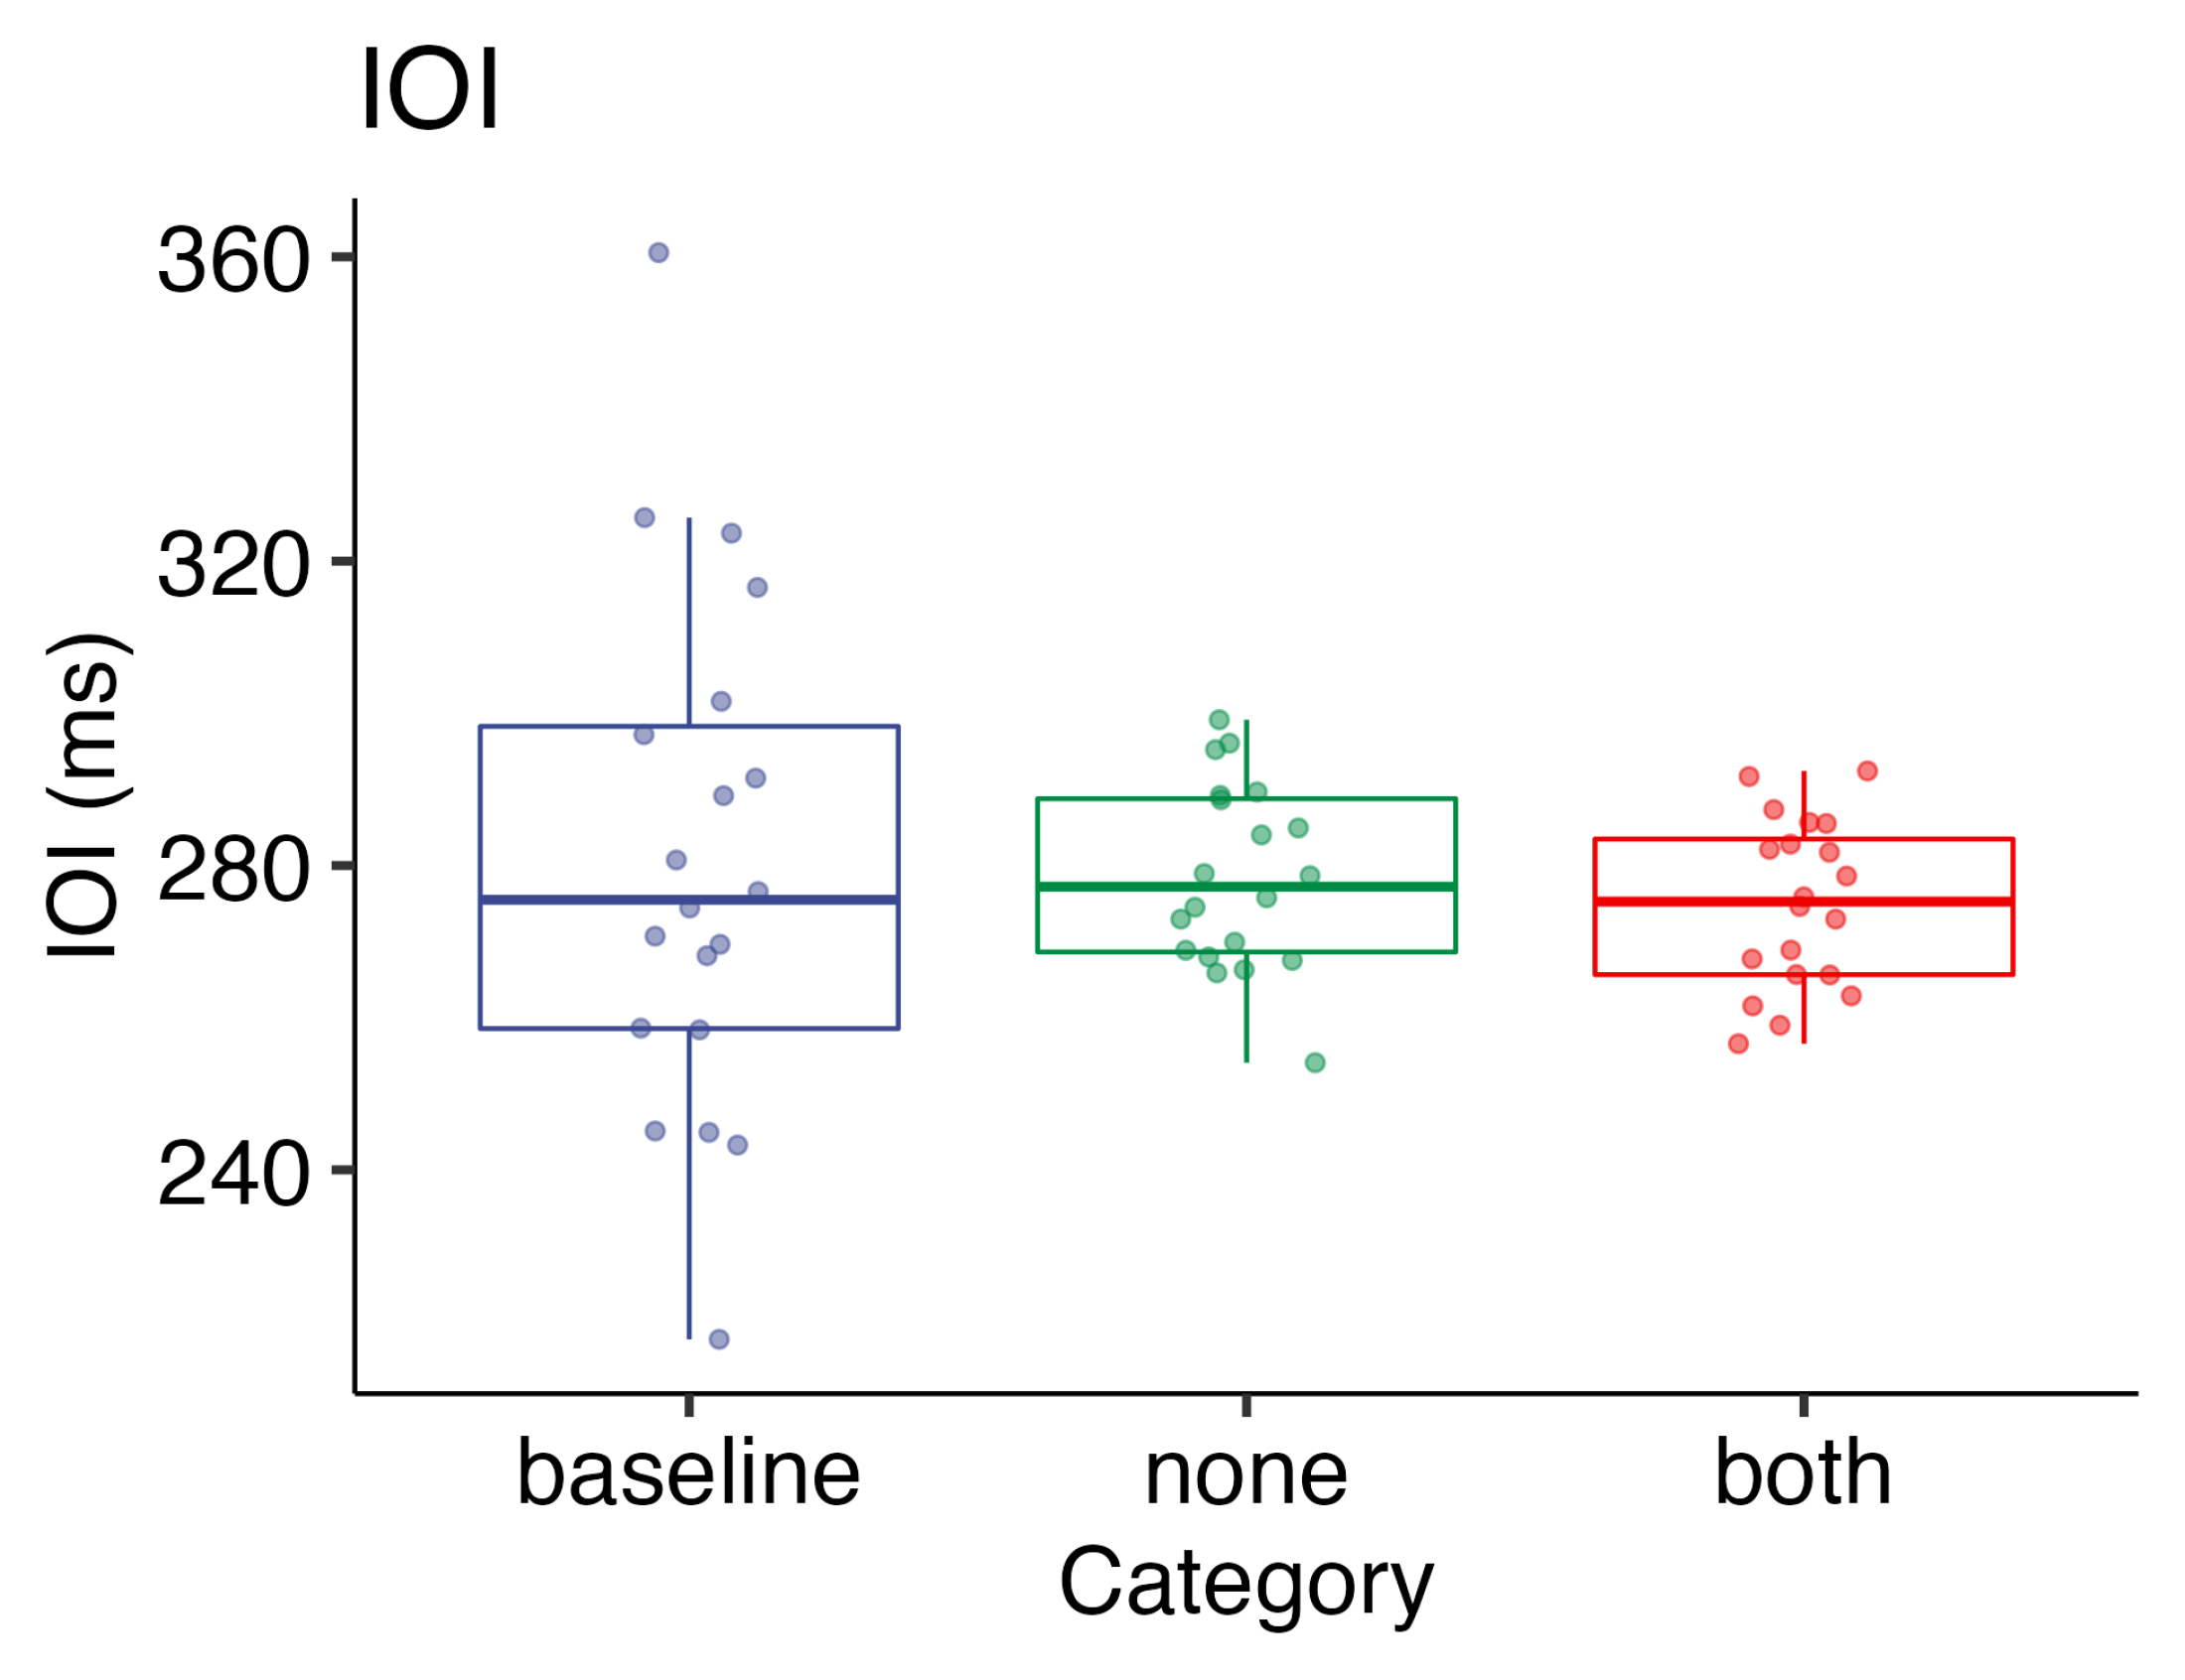
\includegraphics[width=1\linewidth]{manuscript_files/figure-latex/plot-ioi-2-1} \caption{\label{fig:ioi-2}Comparison with the baseline performance in terms of IOIs (ms). A dashed line represents the tempo given by a metronome. Each box indicates the IQR with the median, and whiskers extend to a maximum of 1.5 × IQR beyond the box.}\label{fig:plot-ioi-2}
\end{figure}


\end{document}
